In this chapter, we focus on the negatively confined charged systems, where the dielectric interfaces are characterized by a negative permittivity, leading to a reflection factors that are greater than 1, i.e.,~$\abs{\gamma} > 1$.
Due to the strong polarization effect, the electrostatic interaction in such systems is significantly enhanced compared to the bulk systems and resulting in a failure of the image charge method.
To efficiently simulate such systems, we propose a novel method named the quasi-Ewald method (QEM), which properly accounts for the polarization effect and the long-range interaction in the negatively confined systems.

\section{Quasi-Ewald method}

In this section, we present the quasi-Ewald splitting method, a novel decomposition strategy specifically designed for quasi-2D systems with dielectric interfaces. 
We begin by introducing the quasi-Ewald splitting technique and deriving the Green's function in dielectric confined systems, decomposed into its short-range and long-range components.
We then demonstrate how to efficiently compute electrostatic interactions in positively confined quasi-2D systems by combining this approach with random batch sampling, providing detailed analysis of consistency and variance.
Finally, we introduce a singularity subtraction technique, and extend the QEM to handle negatively confined systems.

% By integrating this approach with random batch sampling, we develop an efficient summation method that achieves linear complexity.
\subsection{Quasi-Ewald splitting}

We start by introducing the quasi-Ewald splitting technique.
Given a fixed point  $\V{r}^\prime=(x^{\prime}, y^{\prime},z^{\prime})$, we decompose   the Dirac delta function into
%%%%%%%%%%%%%%%%%%%%%%%%%%%%%%%%%%%%%%%%%%%%%%%%%%%%%%%%%%
\begin{equation}\label{eq...text...Quasi-EwaldMethod...QuasiEwaldSplitting}
\begin{aligned}
    \delta(\V{r}-\V{r}^\prime) &= \left[\delta (\V{r}-\V{r}^\prime) - {\left( \frac{\alpha}{\pi} \right)} \exp{\left(-\alpha \Norm{\vrho-\vrho^\prime}^2\right)} \delta(z-z^\prime) \right]\\&~~ + {\left( \frac{\alpha}{\pi} \right)} \exp{\left(-\alpha \Norm{\vrho-\vrho^\prime}^2\right)} \delta(z-z^\prime)\;,
    \end{aligned}
\end{equation}
where $\vr:=(\vrho, z):=(x,y,z)$,   $\vrho:=(x,y)$, and $\vrho^\prime:=(x^\prime,y^\prime)$.
 In this formulation, the first term represents  a charge neutral short range kernel centered at $\vr^\prime$, and the second term corresponds to a smooth long range kernel.  We further define  
\begin{equation}\label{eq...text...Kernels}
    \begin{split}
        \sigma_{s}(\V{r}; \vr^\prime) &:= \delta (\V{r}-\V{r}^\prime) - {\left( \frac{\alpha}{\pi} \right)} \exp{\left(-\alpha \Norm{\vrho-\vrho^\prime}^2\right)} \delta(z-z^\prime)\;,\\
        \sigma_{l}(\V{r};\vr^\prime) &:= {\left( \frac{\alpha}{\pi} \right)} \exp{\left(-\alpha \Norm{\vrho-\vrho^\prime}^2\right)} \delta(z-z^\prime)\;,
    \end{split}
\end{equation}
%
%  Consequently, the total charge density in the system can be expressed as 
%
% \begin{equation}
%     \sigma(\vr) = \sum_{\V{m}} \sum_{i = 1}^{N} q_i \left[\sigma_{s}(\V{r} - \V{r}_i + \V{L_m})  +  \sigma_{s}(\V{r} - \V{r}_i + \V{L_m})\right]\;,
% \end{equation}
and  depiction of the decomposition process is provided in Fig.~\ref{fig:QuasiEwaldSplitting}.  
\begin{figure}
    \centering
    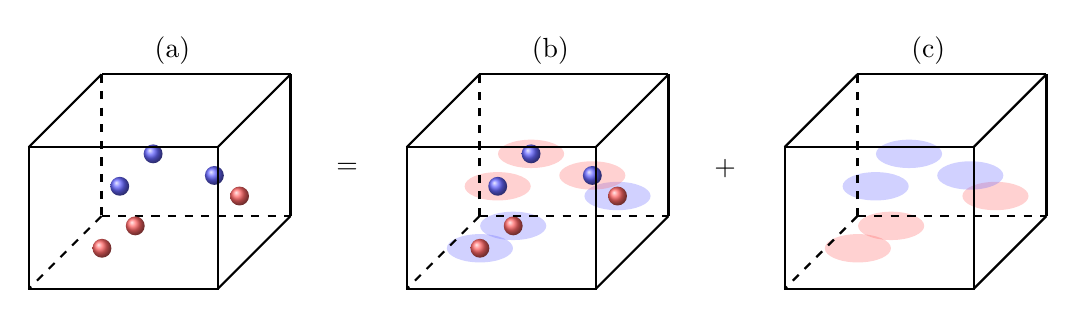
\begin{tikzpicture}[scale = 0.6]

        \def\r{0.2}

        \draw[thick, dashed] (0, 0, 0) -- (4, 0, 0);
        \draw[thick] (4, 0, 0) -- (4, 3, 0);
        \draw[thick] (4, 3, 0) -- (0, 3, 0);
        \draw[thick, dashed] (0, 3, 0) -- (0, 0, 0);


        \foreach \x/\y/\z in {1.1681915835663497/0.4784386449304706/3.0114784670813646, 1.37700874310584/0.4564910752408716/1.723302872827872, 3.730994750135867/1.2345031904085388/2.103105645365449} {
            \shade[ball color=red!60, opacity=1] (\x, \y, \z) circle (\r);
        }

        \foreach \x/\y/\z in {1.827895374334192/2.07357017874381/3.746941345635766, 3.066558538444058/1.5385426337573604/1.7619877149348904, 1.323901301301564/1.5495075401772844/0.6031052215686215} {
            \shade[ball color=blue!60, opacity=1] (\x, \y, \z) circle (\r);
        }

        \draw[thick] (0, 0, 4) -- (4, 0, 4) -- (4, 3, 4) -- (0, 3, 4) -- cycle; % Top face
        \draw[thick, dashed] (0, 0, 0) -- (0, 0, 4); % Front left
        \draw[thick] (4, 0, 0) -- (4, 0, 4); % Front right
        \draw[thick] (4, 3, 0) -- (4, 3, 4); % Back right
        \draw[thick] (0, 3, 0) -- (0, 3, 4); % Back left

        \foreach \x/\y/\z in {1.1681915835663497/0.4784386449304706/3.0114784670813646, 1.37700874310584/0.4564910752408716/1.723302872827872, 3.730994750135867/1.2345031904085388/2.103105645365449} {
            % draw an circle plane laying in the xz plane
            \fill[fill=blue!60, opacity=0.3] (\x + 8, \y, \z) ellipse (0.7 and 0.3);
            \shade[ball color=red!60, opacity=1] (\x + 8, \y, \z) circle (\r);
        }

        \foreach \x/\y/\z in {1.827895374334192/2.07357017874381/3.746941345635766, 3.066558538444058/1.5385426337573604/1.7619877149348904, 1.323901301301564/1.5495075401772844/0.6031052215686215} {
            \fill[fill=red!60, opacity=0.3] (\x + 8, \y, \z) ellipse (0.7 and 0.3);
            \shade[ball color=blue!60, opacity=1] (\x + 8, \y, \z) circle (\r);
        }

        \foreach \x/\y/\z in {1.1681915835663497/0.4784386449304706/3.0114784670813646, 1.37700874310584/0.4564910752408716/1.723302872827872, 3.730994750135867/1.2345031904085388/2.103105645365449} {
            % draw an circle plane laying in the xz plane
            \fill[fill=red!60, opacity=0.3] (\x + 16, \y, \z) ellipse (0.7 and 0.3);
        }

        \foreach \x/\y/\z in {1.827895374334192/2.07357017874381/3.746941345635766, 3.066558538444058/1.5385426337573604/1.7619877149348904, 1.323901301301564/1.5495075401772844/0.6031052215686215} {
            \fill[fill=blue!60, opacity=0.3] (\x + 16, \y, \z) ellipse (0.7 and 0.3);
        }

        \foreach \x/\y/\z in {8/0/0, 16/0/0} {
            \draw[thick, dashed] (\x, \y, \z) -- (4 + \x, \y, \z);
            \draw[thick] (4 + \x, \y, \z) -- (4 + \x, 3 + \y, \z);
            \draw[thick] (4 + \x, 3 + \y, \z) -- (\x, 3 + \y, \z);
            \draw[thick, dashed] (\x, \y, \z) -- (\x, 3 + \y, \z);
            \draw[thick] (\x, \y, 4 + \z) -- (4 + \x, \y, 4 + \z) -- (4 + \x, 3 + \y, 4 + \z) -- (\x, 3 + \y, 4 + \z) -- cycle;
            \draw[thick, dashed] (\x, \y, \z) -- (\x, \y, 4 + \z);
            \draw[thick] (4 + \x, \y, \z) -- (4 + \x, \y, 4 + \z);
            \draw[thick] (4 + \x, 3 + \y, \z) -- (4 + \x, 3 + \y, 4 + \z);
            \draw[thick] (\x, 3 + \y, \z) -- (\x, 3 + \y, 4 + \z);
        }

        \node at (5.2, 1, 0) {$=$};
        \node at (13.2, 1, 0) {$+$};

        \node at (1.5, 3.5, 0) {(a)};
        \node at (9.5, 3.5, 0) {(b)};
        \node at (17.5, 3.5, 0) {(c)};

    \end{tikzpicture}
    \caption{
        An illustration for the quasi-Ewald splitting strategy in a unit cell.
        (a) Charged particles are distributed in the simulation box, cations and anions are represented by red and blue spheres, respectively.
        Sub-figures (b) and (c) shows how Quasi-Ewald splitting works. 
        The discs represent 2D Gaussian charge planes which screen the original point charges.
        We split the original problem into two sub-problems, one with charge neutral particles so that the interactions are short-ranged, another with smooth charge density with a proper geometry so that can be solved rapidly in the reciprocal space.
    }
    \label{fig:QuasiEwaldSplitting}
\end{figure}
Throughout this paper, we will extensively use 2D-Fourier transforms, whose definition is given by
\begin{defination}
    Given function $f(\V{\rho}, z)$, its 2D-Fourier transform is defined by
    \begin{equation}
        \Hat{f}(\V{h}, z):=\int_{\sR^2}f(\V{\rho},z)\exp{(-\mathrm{i} \V{h} \cdot \V{\rho})} d \V{\rho} \;.
    \end{equation}
    The function  $f(\V{\rho}, z)$ can be  recovered from the corresponding inverse 2D-Fourier transform
    \begin{equation} 
        f(\V{\rho}, z)=\frac{1}{4\pi^2}\int_{\sR^2}\Hat{f}(\V{h}, z)\exp{(\mathrm{i} \V{h} \cdot \V{\rho})} d \V{h} \;.
    \end{equation}
\end{defination} 
% \begin{equation}\label{eq...text...FourierTransformKernels}
%     \begin{split}   
%  \hat{\sigma}_{s}(\V{h},z) &=\delta(z)\left[1-\exp\left(-\frac{h^2}{4\alpha}\right)\right]\;,\\
%  \hat{\sigma}_{l}(\V{h},z) &=\delta(z)\exp\left(-\frac{h^2}{4\alpha}\right)\;.
%     \end{split}
% \end{equation}
\begin{prop}
Given fixed point $\V{r}^\prime=(x^{\prime}, y^{\prime},z^{\prime})$, non-zero modes of the 2D-Fourier
transform  of  $ \sigma_{s}(\V{r};\vr^\prime)$ and   $\sigma_{l}(\V{r};\vr^\prime)$  respectively reads
\begin{align*}
 \Hat{\sigma}_{s}(\V{h},z;z^\prime) &= \delta(z-z^\prime) \exp{(-\mathrm{i} \V{h} \cdot \V{\rho}^\prime)}\left(1-\exp\left(-\frac{h^2}{4\alpha}\right)\right)\;,  \\
 \Hat{\sigma}_{l}(\V{h},z;z^\prime) &= \delta(z-z^\prime) \exp{(-\mathrm{i} \V{h} \cdot \V{\rho}^\prime)}\exp\left(-\frac{h^2}{4\alpha}\right)\;,
\end{align*}   
where $\V{h}\neq\vzero$, and the zeroth mode reads
\begin{align*}
 \Hat{\sigma}_{s}(\vzero,z;z^\prime) &= 0\;,  \\
 \Hat{\sigma}_{l}(\vzero,z;z^\prime) &= \delta(z-z^\prime)\;.
\end{align*}   
\end{prop}
\begin{proof}
We observe that for $\V{h}\neq\vzero$, the following integral reads %the  2D-Fourier transform  of $ \sigma_{s}(\V{r}-\vr^\prime)$ reads
\begin{align*}
  % \Hat{\sigma}_{s}(\V{h},z-z^\prime) &=    \int_{\sR^2}\sigma_{s}(\V{r}-\vr^\prime)\exp{(-\mathrm{i} \V{h} \cdot \V{\rho})} d \vrho \\
  % &= \delta(z-z^\prime)\left(
 & \int_{\sR^2}\left[\delta(\vrho-\vrho^\prime)- {\left( \frac{\alpha}{\pi} \right)} \exp{\left(-\alpha \Norm{\vrho-\vrho^\prime}^2\right)}\right] \exp{(-\mathrm{i} \V{h} \cdot \V{\rho})} d \vrho \\
 =&\exp{(-\mathrm{i} \V{h} \cdot \V{\rho}^\prime)}\left[1-  \int_{\sR^2}{\left( \frac{\alpha}{\pi} \right)} \exp{\left(-\alpha \Norm{\vrho-\vrho^\prime}^2\right)}  \exp{(-\mathrm{i} \V{h} \cdot (\V{\rho}-\vrho^\prime))} d \vrho\right]\\
 =&\exp{(-\mathrm{i} \V{h} \cdot \V{\rho}^\prime)}\left(1-\exp\left(-\frac{h^2}{4\alpha}\right)\right)\;,
\end{align*}
hence we obtain that 
\begin{align*}
 \Hat{\sigma}_{s}(\V{h},z;z^\prime) &= \delta(z-z^\prime) \exp{(-\mathrm{i} \V{h} \cdot \V{\rho}^\prime)}\left(1-\exp\left(-\frac{h^2}{4\alpha}\right)\right)\;,  \\
 \Hat{\sigma}_{l}(\V{h},z;z^\prime) &= \delta(z-z^\prime) \exp{(-\mathrm{i} \V{h} \cdot \V{\rho}^\prime)}\exp\left(-\frac{h^2}{4\alpha}\right)\;.
\end{align*}
We observe further that the following integral reads
\begin{align*}
  % \Hat{\sigma}_{s}(\V{h},z-z^\prime) &=    \int_{\sR^2}\sigma_{s}(\V{r}-\vr^\prime)\exp{(-\mathrm{i} \V{h} \cdot \V{\rho})} d \vrho \\
  % &= \delta(z-z^\prime)\left(
 & \int_{\sR^2}\left[\delta(\vrho-\vrho^\prime)- {\left( \frac{\alpha}{\pi} \right)} \exp{\left(-\alpha \Norm{\vrho-\vrho^\prime}^2\right)}\right]  d \vrho \\
 =&\int_{\sR^2}\left[\delta(\vrho-\vrho^\prime)- {\left( \frac{\alpha}{\pi} \right)} \exp{\left(-\alpha \Norm{\vrho-\vrho^\prime}^2\right)}\right]  d \left(\vrho-\vrho^\prime\right) =0\;,
\end{align*}
which finishes the proof.
\end{proof}
% Given $\vr_0:=(\vrho_0,z_0):=(x_0, y_0, z_0)\in\Omega_{\mrm{c}}$,  then the   Poisson's equation reads 
% \begin{equation}\label{eq...text...RepPoisson}
%     \left \{
%     \begin{array}{ll}
%         - \grad_{\V{r}} \cdot\left[ \epsilon(\V{r}) \grad_{\V{r}} G(\V{r},~\V{r}_0) \right] = \delta (\V{r} - \V{r}_0), & \V r \in \mathbb{R}^3 \;, \\
% %%%%%%%%%%%%%%%%%%%%%%%%%%%        
%         G(\V{r},~\V{r}_0) |_{-} = G(\V{r},~\V{r}_0) |_{+}, & \text{on}~\partial\Omega_{\mrm{c}}\;, \\
% %%%%%%%%%%%%%%%%%%%%%%%%%%%        
%           \partial_{z} G(\V{r},~\V{r}_0) |_{-} = \epsilon_{\mrm{u}} \partial_{z} G(\V{r},~\V{r}_0) |_{+}, & \text{on}~\partial \Omega_{\mrm{c}} \cap \partial \Omega_{\mrm{u}}\;,     \\
% %%%%%%%%%%%%%%%%%%%%%%%%%%%            
%   \partial_{z} G(\V{r},~\V{r}_0) |_{-} = \epsilon_{\mrm{d}} \partial_{z} G(\V{r},~\V{r}_0) |_{+}, & \text{on}~\partial \Omega_{\mrm{c}} \cap \partial \Omega_{\mrm{d}}\;,\\
% %%%%%%%%%%%%%%%%%%%%%%%%%%%  
% G(\V{r},~\V{r}_0) \to 0, & \text{as}~{r} \to \infty\;.
% \end{array}\right.
% \end{equation}


Then by employing the Dirichlet to Neumann mapping technique to the Poisson's equation Eq.~\eqref{eq:Poisson_G}, we can derive the Green's function~$G(\V{r}, \V{r_0})$ in the reciprocal space. 

\begin{thm}\label{Proposition...GreensFunction}
    As we define
    \begin{equation}
        \Hat{G}(\V{h}, z; z_0) = \int_{\mathbb{R}^2} G(\V{r}, \V{r_0}) \exp{(-\mathrm{i} \V{h} \cdot \V{\rho})} d \vrho\;,
    \end{equation}     
then for $\V{h}=\vzero$,   
\begin{equation}\label{eq...hat_G_solution...Zeroth}
        \hat{G}(\vzero, z; z_0) = \frac{\abs{z-z_0}}{2}\;,
\end{equation}        
and for $\V{h}\neq \vzero$,     
    \begin{equation}\label{eq...hat_G_solution...Non-zero}
    \begin{aligned}
\hat{G}(\V{h}, z; z_0) &=  \frac{ \exp{(-\mathrm{i} \V{h} \cdot \V{\rho}_0)}}{2 h  \left(1-\gamma_{\mrm{u}}\gamma_{\mrm{d}}\exp(-2 h H)\right)} \sum_{p=1}^4\Gamma_p\exp(- h a_p(z;z_0))\;, %\Big[\exp(-h\abs{z-z_0})\\
% &~~+\gamma_{\mrm{d}}\exp(-h(z+z_0))+\gamma_{\mrm{u}}\exp(-h(2H-z-z_0))\\
% &~~+\gamma_{\mrm{u}}\gamma_{\mrm{d}}\exp(-h(2H-\abs{z-z_0}))\Big]\;.
    \end{aligned}     
    \end{equation}         
where 
\begin{align*}
 \Gamma_{1:4}&:=\left[1,\gamma_{\mrm{d}},\gamma_{\mrm{u}},\gamma_{\mrm{u}}\gamma_{\mrm{d}}\right]\;,\\
 a_{1:4}(z;z_0)&:=\left[\abs{z-z_0}, z+z_0,2H-z-z_0,2H-\abs{z-z_0}\right]\;.
\end{align*}
\end{thm}
\begin{proof}
    By applying Fourier transform on both sides of Eq.~\eqref{eq:Poisson_G}, then for $\V{h}\neq \vzero$, i.e., $k>0$, we obtain that
    \begin{equation*} 
        \begin{split}
            \frac{\partial^2 \Hat{G}_{\mrm{c}}(\V{h}, z; z_0)}{{\partial z}^2} - h^2 \Hat{G}_{\mrm{c}}(\V{h}, z; z_0) = - \frac{ \exp{(-\mathrm{i} \V{h} \cdot \V{\rho}_0)}\delta (z- z_0)}{ }&,~z \in [0, H],\\
            \frac{\partial^2 \hat{G}_{\mrm{u}}(\V{h}, z; z_0)}{{\partial z}^2} - h^2 \hat{G}_{\mrm{u}}(\V{h}, z; z_0) = 0&,~z > H,\\
            \frac{\partial^2 \hat{G}_{\mrm{d}}(\V{h}, z; z_0)}{{\partial z}^2} - h^2 \hat{G}_{\mrm{d}}(\V{h}, z; z_0) = 0&,~z < 0,
        \end{split}
    \end{equation*}
    with the boundary conditions satisfying    
    \begin{equation*}
        \begin{split}
            \Hat{G}_{\mrm{c}}(\V{h}, 0; z_0) &= \Hat{G}_{\mrm{d}}(\V{h}, 0; z_0)\;,\\
            \hat{G}_{\mrm{c}}(\V{h}, H; z_0) &= \hat{G}_{\mrm{u}}(\V{h}, H; z_0)\;,\\
              \partial_z\Hat{G}_{\mrm{c}}(\V{h}, 0; z_0) &= \epsilon_{\mrm{d}} \partial_z\Hat{G}_{\mrm{d}}(\V{h}, 0; z_0)\;,\\
              \partial_z\Hat{G}_{\mrm{c}}(\V{h}, H; z_0) &= \epsilon_{\mrm{u}} \partial_z\Hat{G}_{\mrm{u}}(\V{h}, H; z_0)\;,\\
            \lim_{z \to \infty} \Hat{G}_{\mrm{u}}(\V{h}, z; z_0) &= \lim_{z \to -\infty}\Hat{G}_{\mrm{d}}(\V{h}, z; z_0)  = 0\;,
        \end{split}
    \end{equation*}
based on the infinite boundary condition,  $\Hat{G}_{\mrm{u}}(\V{h}, z; z_0)$ and $\Hat{G}_{\mrm{d}}(\V{h}, z; z_0)$ take the form
\begin{align*}
    \Hat{G}_{\mrm{u}}(\V{h}, z; z_0)&=C_{\mrm{u}}(z_0)\exp(- h z),~z > H\;,\\
     \Hat{G}_{\mrm{d}}(\V{h}, z; z_0)&=C_{\mrm{d}}(z_0)\exp(h z),~~~~z < 0\;,
\end{align*}
therefore, we have 
\begin{align*}
    \partial_z\Hat{G}_{\mrm{u}}(\V{h}, z; z_0)&=-k\Hat{G}_{\mrm{u}}(\V{h}, z; z_0),~z > H\;,\\
     \partial_z\Hat{G}_{\mrm{d}}(\V{h}, z; z_0)&=k\Hat{G}_{\mrm{d}}(\V{h}, z; z_0),~z < 0\;,
\end{align*}
hence the boundary condition can be  simplified into
\begin{align*}
  \partial_z\Hat{G}_{\mrm{c}}(\V{h}, 0; z_0)&=\epsilon_{\mrm{d}} \partial_z\Hat{G}_{\mrm{d}}(\V{h}, 0; z_0)=k\epsilon_{\mrm{d}} \Hat{G}_{\mrm{d}}(\V{h}, 0; z_0)=k\epsilon_{\mrm{d}} \Hat{G}_{\mrm{c}}(\V{h}, 0; z_0)\;,\\
   \partial_z\Hat{G}_{\mrm{c}}(\V{h}, H; z_0)&=\epsilon_{\mrm{u}} \partial_z\Hat{G}_{\mrm{u}}(\V{h}, H; z_0)=-k\epsilon_{\mrm{u}} \Hat{G}_{\mrm{u}}(\V{h}, H; z_0)=-k\epsilon_{\mrm{u}} \Hat{G}_{\mrm{c}}(\V{h}, H; z_0)\;.
\end{align*} 
Finally, for $z\in[0, z_0]$, $\Hat{G}_{\mrm{c}}(\V{h}, z; z_0)$ takes the form
\begin{equation*}
    \Hat{G}_{\mrm{c}}(\V{h}, z; z_0)=\left \{
            \begin{array}{cc}
                \begin{aligned}
                    & A\exp(h z)+B\exp(-h z)\;,
                \end{aligned} & z>z_0, \\
                \begin{aligned}
                 & E\exp(h z)+F\exp(-h z)\;,
                \end{aligned} & z<z_0,
            \end{array}
        \right. \;
\end{equation*}
with $A, B, E, F$ satisfying
\begin{equation}\label{proof...Matrix}
\begin{aligned}
 &A\exp(hz_0)+B\exp(-hz_0)  = E\exp(hz_0)+F\exp(-hz_0)\;,\\
 &A\exp(hz_0)-B\exp(-hz_0)-E\exp(hz_0)+F\exp(-hz_0)=-\frac{ \exp{(-\mathrm{i} \V{h} \cdot \V{\rho}_0)}}{h }\;,\\
 & (E-F)=\epsilon_{\mrm{d}}(E+F)\;,\\
 & \left(A\exp(hH)-B\exp(-hH)\right)=-\epsilon_{\mrm{u}}\left(A\exp(hH)+B\exp(-hH)\right)\;,
\end{aligned}\end{equation}
whose solution reads
\begin{align*}
A&=\frac{ \exp{(-\mathrm{i} \V{h} \cdot \V{\rho}_0)}}{2h }\frac{\exp(-2hH)}{1-\gamma_{\mrm{u}}\gamma_{\mrm{d}}\exp(-2hH)} \left(\gamma_{\mrm{u}}\exp(hz_0)+\gamma_{\mrm{u}}\gamma_{\mrm{d}}\exp(-hz_0)\right)\;,\\
B&=\frac{ \exp{(-\mathrm{i} \V{h} \cdot \V{\rho}_0)} }{2h }\frac{1}{1-\gamma_{\mrm{u}}\gamma_{\mrm{d}}\exp(-2hH)} \left(\exp(hz_0)+\gamma_{\mrm{d}}\exp(-hz_0)\right)\;,\\
E&=A+\frac{\exp{(-\mathrm{i} \V{h} \cdot \V{\rho}_0)} }{2h }\exp(-hz_0)\\
&=\frac{\exp{(-\mathrm{i} \V{h} \cdot \V{\rho}_0)}}{2h }\frac{\gamma_{\mrm{u}}\exp(-2hH)}{1-\gamma_{\mrm{u}}\gamma_{\mrm{d}}\exp(-2hH)} \exp(hz_0)\\&~~+\frac{\exp{(-\mathrm{i} \V{h} \cdot \V{\rho}_0)}}{2h }\frac{1}{1-\gamma_{\mrm{u}}\gamma_{\mrm{d}}\exp(-2hH)}\exp(-hz_0)\;,\\
F&=\frac{\exp{(-\mathrm{i} \V{h} \cdot \V{\rho}_0)}}{2h }\frac{\gamma_{\mrm{u}}\gamma_{\mrm{d}}\exp(-2hH)}{1-\gamma_{\mrm{u}}\gamma_{\mrm{d}}\exp(-2hH)} \exp(hz_0)\\&~~+\frac{\exp{(-\mathrm{i} \V{h} \cdot \V{\rho}_0)}}{2h }\frac{\gamma_{\mrm{d}}}{1-\gamma_{\mrm{u}}\gamma_{\mrm{d}}\exp(-2hH)} \exp(-hz_0)\;,
\end{align*}
 and similar procedures can be applied to the case $\V{h}=\vzero$, we omit this for brevity.
\end{proof}

\begin{rmk}\label{Remark...Nonzero+larger}
    If $\gamma_u \gamma_d < 1$, the determinant of the Eq.~\eqref{proof...Matrix} is non-zero on the positive real axis.
    However, for negatively confined systems with $\gamma_u \gamma_d > 1$, a first order pole exists at $k_0 = \ln(\gamma_u \gamma_d)/2H$ and the Green's function diverges.
    Moreover, it is noteworthy that all the components in $a_{1:4}(z;z_0)$ take positive values. 
\end{rmk}


Based on the decomposition relation Eq.~\eqref{eq...text...Quasi-EwaldMethod...QuasiEwaldSplitting} and definition in Eq.~\eqref{eq...text...Kernels}, we observe that 
\begin{equation}%\label{eq...text...Rewrite-in-kernels}
   \delta(\V{r}-\V{r}_0)=\sigma_s  (\V{r};\V{r}_0)+\sigma_\ell  (\V{r};\V{r}_0)\;,
\end{equation}
and we  shall decompose the Green's function  $ G(\V{r}, \V{r_0})$ correspondingly into
\begin{equation}
    G(\V{r}, \V{r_0})= G_s(\V{r}, \V{r_0})+  G_\ell(\V{r}, \V{r_0})\;,
\end{equation}
where $ G_s(\V{r}, \V{r_0})$ and $  G_\ell(\V{r}, \V{r_0})$ are the solutions to the Poisson's equation Eq.~\eqref{eq:Poisson_G} except that $\delta(\V{r}-\V{r}_0)$ is replaced respectively by $\sigma_s  (\V{r};\V{r}_0)$ and $\sigma_\ell  (\V{r};\V{r}_0)$.
\begin{corollary}
For any $\V{h}\neq \vzero$, given     $\hat{G}(\V{h}, z; z_0)$, we obtain that  
    \begin{align*}
        \hat{G}_s(\V{h}, z; z_0)&=\hat{G}(\V{h}, z; z_0)\left[1-\exp\left(-\frac{h^2}{4\alpha}\right)\right]\;,\\
        \hat{G}_\ell(\V{h}, z; z_0)&=\hat{G}(\V{h}, z; z_0)\exp\left(-\frac{h^2}{4\alpha}\right)\;,
    \end{align*} 
    and for  $\V{h}=\vzero$, given     $\hat{G}(\vzero, z; z_0)$, we obtain that  
        \begin{align*}
        \hat{G}_s(\vzero, z; z_0)&=0\;,\\
        \hat{G}_\ell(\vzero, z; z_0)&=\hat{G}(\vzero, z; z_0)\;.
    \end{align*} 
\end{corollary}
Its proof is straightforward in that we only need to solve out the Systems of Eq.~\eqref{proof...Matrix} by replacing  the coefficient $-\frac{\exp{(-\mathrm{i} \V{h} \cdot \V{\rho}_0)}}{h }$ with  
\begin{equation*}
    -\frac{\exp{(-\mathrm{i} \V{h} \cdot \V{\rho}_0)}}{h }\left[1-\exp\left(-\frac{h^2}{4\alpha}\right)\right]\;,
\end{equation*}
and 
\begin{equation*}
    -\frac{\exp{(-\mathrm{i} \V{h} \cdot \V{\rho}_0)}}{h }\exp\left(-\frac{h^2}{4\alpha}\right)\;,
\end{equation*} 
respectively.
Consequently, the Green's function $ G_s(\V{r}, \V{r_0})$ and $  G_\ell(\V{r}, \V{r_0})$ can be recovered following the inverse Fourier transform of $  \hat{G}_s(\V{h}, z; z_0)$ and $  \hat{G}_\ell(\V{h}, z; z_0)$,
\begin{equation*}
\begin{aligned}
 G_s(\V{r}, \V{r_0})&=   \frac{1}{4\pi^2}\int_{\sR^2} \hat{G}_s(\V{h}, z; z_0)\exp{(\mathrm{i} \V{h} \cdot \V{\rho})} d \V{h}\\
 &= \frac{1}{4\pi^2}\int_{\sR^2} \hat{G}(\V{h}, z; z_0)\left[1-\exp\left(-\frac{h^2}{4\alpha}\right)\right]\exp{(\mathrm{i} \V{h} \cdot \V{\rho})} d \V{h}\;,\\
  G_\ell(\V{r}, \V{r_0})&=   \frac{1}{4\pi^2}\int_{\sR^2} \hat{G}_\ell(\V{h}, z; z_0)\exp{(\mathrm{i} \V{h} \cdot \V{\rho})} d \V{h}\\
 &= \frac{1}{4\pi^2}\int_{\sR^2} \hat{G}(\V{h}, z; z_0)\exp\left(-\frac{h^2}{4\alpha}\right)\exp{(\mathrm{i} \V{h} \cdot \V{\rho})} d \V{h}\;.
\end{aligned}    
\end{equation*}
Hence the total interaction energy reads
\begin{align*}
   U & =   U_s+U_\ell\;,
\end{align*}
whereas
\begin{align}
U_s&:=    \frac{1}{2} {\sum_{\V{m}}}^\prime \sum_{i, j = 1}^{N} q_i q_j G_s(\V{r}_i+\vL_m, \V{r}_j)\;, \label{eq::U_s}\\
U_\ell&:=   \frac{1}{2} {\sum_{\V{m}}}\sum_{i, j = 1}^{N} q_i q_j  G_\ell(\V{r}_i+\vL_m, \V{r}_j)\;. \label{eq::U_l}
\end{align}
Given $\vr_j:=(\vrho_j, z_j)$, then for the short range kernel $G_s(\cdot, \V{r}_j)$, whose expression reads 
\begin{align*}
 &G_s(\V{r}, \V{r}_j)\\
 =&   \frac{1}{4\pi^2}\int_{\sR^2} \hat{G}(\V{h}, z; z_j)\left[1-\exp\left(-\frac{h^2}{4\alpha}\right)\right]\exp{(\mathrm{i} \V{h} \cdot \V{\rho})} d \V{h}\\
 =& \frac{1}{4\pi^2}\int_{\sR^2} \frac{ \exp{(\mathrm{i} \V{h} \cdot (\V{\rho}-\V{\rho}_j))}}{2h \left(1-\gamma_{\mrm{u}}\gamma_{\mrm{d}}\exp(-2hH)\right)} \left[1-\exp\left(-\frac{h^2}{4\alpha}\right)\right]\left[\sum_{p=1}^4\Gamma_p\exp(-ha_p(z;z_j))\right]d \V{h}\;,
% =&\frac{1}{8\pi^2 }\int_{\sR^2} \frac{ \exp{(\mathrm{i} \V{h} \cdot \V{\rho}_{ij})}}{k\left(1-\gamma_{\mrm{u}}\gamma_{\mrm{d}}\exp(-2hH)\right)} \left[1-\exp\left(-\frac{h^2}{4\alpha}\right)\right]\sum_{p=1}^4\Gamma_p\exp(-ha_p(z_i;z_j))d \V{h}\;,
\end{align*}
moreover, if further given $\V{r}_i:=(\vrho_i, z_i)$, we obtain that 
\begin{align*}
   &G_s(\V{r}_i, \V{r}_j)\\
   =& \frac{1}{8\pi^2 }\int_{\sR^2} \frac{ \exp{(\mathrm{i} \V{h} \cdot \V{\rho}_{ij})}}{k\left(1-\gamma_{\mrm{u}}\gamma_{\mrm{d}}\exp(-2hH)\right)} \left[1-\exp\left(-\frac{h^2}{4\alpha}\right)\right]\left[\sum_{p=1}^4\Gamma_p\exp(-ha_p(z_i;z_j))\right]d \V{h}\;,
\end{align*}
where $\V{\rho}_{ij}:=\vrho_i-\vrho_j$. 
In actually calculations, due to the short range nature of~$G_s(\cdot, \V{r}_j)$, the infinite sum in Eq.~\eqref{eq::U_s} is truncated to a finite sum in real space with a cutoff $r_c$, given by
\begin{equation}\label{eq::U_s_truncated}
    U_s \approx U_{s, *} = \sum_{\abs{\bm{\rho}_{ij, m}} \leq r_c} q_i q_j G_s(\V{r}_i+\vL_m, \V{r}_j)\;,
\end{equation}
where $\bm{\rho}_{ij, m}:=\vrho_i-\vrho_j+ (L_x m_x, L_y m_y)$, and the summation indicates that among all possible pairs of particles, only the terms with $\abs{\bm{\rho}_{ij, m}} \leq r_c$ are considered.


 As for the long  range kernel $ G_\ell(\cdot, \V{r}_j)$, based on the Poisson summation formula, we obtain that 
% \begin{align*}
%  & G_\ell(\V{r}_i, \V{r}_j)\\
%  =&   \frac{1}{4\pi^2}\int_{\sR^2} \hat{G}(\V{h}, z_i; z_j)\exp\left(-\frac{h^2}{4\alpha}\right)\exp{(\mathrm{i} \V{h} \cdot \V{\rho}_i)} d \V{h}\\
%  =& \frac{1}{4\pi^2}\int_{\sR^2} \frac{ \exp{(\mathrm{i} \V{h} \cdot (\V{\rho}_i-\V{\rho}_j))}}{2h \left(1-\gamma_{\mrm{u}}\gamma_{\mrm{d}}\exp(-2hH)\right)} \exp\left(-\frac{h^2}{4\alpha}\right)\sum_{p=1}^4\Gamma_p\exp(-ha_p(z_i;z_j))d \V{h}\\
%  =&\frac{1}{8\pi^2 }\int_{\sR^2} \frac{ \exp{(\mathrm{i} \V{h} \cdot \V{\rho}_{ij})}}{k\left(1-\gamma_{\mrm{u}}\gamma_{\mrm{d}}\exp(-2hH)\right)} \exp\left(-\frac{h^2}{4\alpha}\right)\sum_{p=1}^4\Gamma_p\exp(-ha_p(z_i;z_j))d \V{h}\;,
% \end{align*}
\begin{equation}\label{eq...text...PoissonSummation}
 \sum_{\vm}  G_\ell(\V{r}+\vL_m, \V{r}_j)  =\frac{1}{ L_xL_y}   \sum_{\V{h}\in\fK^2} \Hat{G}_\ell(\V{h},z;z_j)\exp(\textrm{i}\V{h}\cdot \vrho) \;,
\end{equation}
where \[\fK^2 := \left\{\V{h} \in \frac{  2\pi}{L_x}\sZ\times \frac{  2\pi}{L_y}\sZ \right\}\;.\]
Furthermore, the RHS of Eq. \eqref{eq...text...PoissonSummation} reads
\begin{align*}
&\frac{1}{ L_xL_y}   \sum_{\V{h}\in\fK^2} \Hat{G}_\ell(\V{h},z;z_j)\exp(\textrm{i}\V{h}\cdot \vrho)\\
%=&\frac{1}{ L_xL_y}  \left( \sum_{\V{h}\in\fK^2}  \hat{G}(\V{h}, z; z_j)\exp\left(-\frac{h^2}{4\alpha}\right)\exp{(\mathrm{i} \V{h} \cdot \V{\rho})} \right)\\
=& \frac{1}{ L_xL_y}   \left[\Hat{G}_\ell(\vzero, z; z_j)+\sum_{\V{h}\in\fK^2,\V{h}\neq\vzero}  \hat{G}_\ell(\V{h}, z; z_j)\exp{(\mathrm{i} \V{h} \cdot \V{\rho})}\right]\\
=&\frac{1}{ L_xL_y}   \left[\hat{G}(\vzero, z; z_j)+\sum_{\V{h}\in\fK^2,\V{h}\neq\vzero}  \hat{G}(\V{h}, z; z_j)\exp\left(-\frac{h^2}{4\alpha}\right)\exp{(\mathrm{i} \V{h} \cdot \V{\rho})}\right]\;,
\end{align*}
therefore, given $\vr_i$, the above expression can be simplified into
\begin{align*}
 &\frac{1}{ L_xL_y}   \sum_{\V{h}\in\fK^2,\V{h}\neq\vzero} \Hat{G}_\ell(\V{h},z;z_j)\exp(\textrm{i}\V{h}\cdot \vrho)\\
 =& \frac{1}{ L_xL_y}   \sum_{\V{h}\in\fK^2,\V{h}\neq\vzero} \frac{ \exp{(\mathrm{i} \V{h} \cdot \V{\rho}_{ij})}}{2h \left(1-\gamma_{\mrm{u}}\gamma_{\mrm{d}}\exp(-2hH)\right)}\left[\sum_{p=1}^4\Gamma_p\exp(-ha_p(z_i;z_j))\right] \exp\left(-\frac{h^2}{4\alpha}\right)\;,
\end{align*}
to sum up, the energy $U_\ell$ reads
\begin{align*}
    U_\ell&=\frac{1}{2}\sum_{\vm}\sum_{i,j=1}^N q_iq_j G_\ell(\V{r}_i+\vL_m, \V{r}_j)\\
    &=\frac{1}{4  L_xL_y}\sum_{i,j=1}^N  q_iq_j \Bigg({\Abs{z_i-z_j}} +\\&~~~~+  \sum_{\V{h}\in\fK^2,\V{h}\neq\vzero} \frac{ \exp{(\mathrm{i} \V{h} \cdot \V{\rho}_{ij})}}{k\left(1-\gamma_{\mrm{u}}\gamma_{\mrm{d}}\exp(-2hH)\right)}\left[\sum_{p=1}^4\Gamma_p\exp(-ha_p(z_i;z_j))\right] \exp\left(-\frac{h^2}{4\alpha}\right)\Bigg)\;.
\end{align*}


\subsection{The algorithm}

We first consider the case where the dielectric constants of the upper and lower regions are positive, i.e., $\gamma_{\mrm{u}} \gamma_{\mrm{d}} < 1$. 
We develop fast algorithms for numerically evaluating both the short-range and long-range parts of the interaction energy.

First we consider the short-range part $U_s$.
We observe that the energy $U_s$ is constituted by the terms
\begin{align*}
  &G_s(\V{r}_i, \V{r}_j)\\
   =& \frac{1}{8\pi^2 }\int_{\sR^2} \frac{ \exp{(\mathrm{i} \V{h} \cdot \V{\rho}_{ij})}}{h \left(1-\gamma_{\mrm{u}}\gamma_{\mrm{d}}\exp(-2hH)\right)} \left[1-\exp\left(-\frac{h^2}{4\alpha}\right)\right]\left[\sum_{p=1}^4\Gamma_p\exp(-ha_p(z_i;z_j))\right]d \V{h}\;,  
\end{align*}
in which $\vr_i$ and $\vr_j$ are given, and we further notice  that all the components in $G_s(\V{r}_i, \V{r}_j)$ take the form
\begin{equation}\label{eq::int_Gs}
    \begin{split}
        & \int_{\sR^2} \frac{ \exp{(\mathrm{i} \V{h} \cdot \V{\rho}_{ij})}}{h \left(1-\gamma_{\mrm{u}}\gamma_{\mrm{d}}\exp(-2hH)\right)} \left[1-\exp\left(-\frac{h^2}{4\alpha}\right)\right]\exp(-ha_p(z_i;z_j))d \V{h}\\
        =2\pi&\int_0^{+\infty} \frac{ \exp(-ha_p(z_i;z_j))}{1-\gamma_{\mrm{u}}\gamma_{\mrm{d}}\exp(-2hH)} \left[1-\exp\left(-\frac{h^2}{4\alpha}\right)\right] J_0(\rho_{ij}k)d k\;,
    \end{split}
\end{equation}
where $\rho_{ij}:=\Norm{\vrho_{ij}}=\Norm{\vrho_i-\vrho_j}$, and $ J_0(\cdot)$ is the zeroth-order Bessel function,  which  can   be expressed as a complex contour integral over a full period.
\begin{defination}
    The zeroth-order Bessel function of the first kind, denoted by $ J_0(r)$, is formally defined via the integral representation
\begin{equation}
       J_0(r):=\frac{1}{2\pi} \int_0^{2\pi} \exp(\mathrm{i} r\sin \theta) d \theta\;.  
    \end{equation}
\end{defination}
We proceed to evaluate the following integral
\begin{equation}\label{eq...text...InfiniteIntegral}
\int_0^{+\infty} \frac{ \exp(-ah)}{1-\gamma_{\mrm{u}}\gamma_{\mrm{d}}\exp(-2hH)} \left[1-\exp\left(-\frac{h^2}{4\alpha}\right)\right] J_0(\rho h)d k\;,    
\end{equation}
where $a>0$ and $\rho>0$ are fixed constants. Firstly, we observe that Eq. \eqref{eq...text...InfiniteIntegral} can be written into
\begin{align*}
   & \int_0^{+\infty} \frac{ \exp(-ah)}{1-\gamma_{\mrm{u}}\gamma_{\mrm{d}}\exp(-2hH)} \left[1-\exp\left(-\frac{h^2}{4\alpha}\right)\right] J_0(\rho h)d k\\
   =&\underbrace{\int_0^{+\infty} \frac{1}{1-\gamma_{\mrm{u}}\gamma_{\mrm{d}}\exp(-2hH)}  \exp(-ah)  J_0(\rho h)d k}_{\text{Term}~\mathrm{I}}\\
   &-\underbrace{\int_0^{+\infty} \frac{1}{1-\gamma_{\mrm{u}}\gamma_{\mrm{d}}\exp(-2hH)}\exp\left(-\frac{h^2}{4\alpha}\right)  \exp(-ah)  J_0(\rho h)d k}_{\text{Term}~\mathrm{II}}\;.
\end{align*}
Secondly, we observe further that Term $\mathrm{I}$ can be decomposed into
\begin{align*}
&\int_0^{+\infty} \frac{1}{1-\gamma_{\mrm{u}}\gamma_{\mrm{d}}\exp(-2hH)}  \exp(-ah)  J_0(\rho h)d k\\
=&\underbrace{\int_0^{+\infty}   \exp(-ah)  J_0(\rho h)d k}_{\text{Term}~\mathrm{I(a)}}\\
&+\underbrace{\int_0^{+\infty} \frac{\gamma_{\mrm{u}}\gamma_{\mrm{d}}}{1-\gamma_{\mrm{u}}\gamma_{\mrm{d}}\exp(-2hH)}  \exp(-2hH)\exp(-ah)  J_0(\rho h)d k}_{\text{Term}~\mathrm{I(b)}}\;,
\end{align*}
on the basis of the identity
\begin{equation*}
    \int_0^{+\infty}\exp(-ax) J_0(x)d x=\frac{1}{\sqrt{a^2+1}}\;,
\end{equation*}
then Term $\mathrm{I(a)}$ can be simplified into 
\begin{equation}\label{eq...text...TermI(A)}
    \int_0^{+\infty}   \exp(-ah)  J_0(\rho h)d k=\frac{1}{\sqrt{a^2+\rho^2}}\;.
\end{equation}
It is observed that Term $\mathrm{I(b)}$ and Term $\mathrm{II}$  comprise infinite integrals involving rapidly decaying functions coupled with oscillatory components. To efficiently evaluate such integrals over an infinite domain, we employ the method proposed in \cite{trefethen2022exactness}, which facilitates numerical computation by truncating the integration region to a finite domain. 
% \begin{thm}[Theorem 5.1 in \cite{trefethen2022exactness}]\label{Thm...Truncation}
%  Let $f(x)$ be analytic and bounded for $x \in(-\infty, \infty)$, and suppose $F(x):=\exp \left(-x^2\right) f(x)$ extends to a bounded analytic function in the infinite strip $-a<\operatorname{Im} x<$ a for some $a>0$. Let $L>0$ be fixed, and for each $n \geq 1$, as we denote  \[I_n(F):=\sum_{j=1}^n w_jF(x_j)\;,\] as the estimate of the integral \[I(F):=\int_{-\infty}^{+\infty} F(x)d x \;,\]  obtained by applying Gauss-Legendre, Clenshaw-Curtis, or equispaced trapezoidal quadrature on the truncated interval $\left[-L n^{1 / 3}, L n^{1 / 3}\right]$. Then for some $C>0$,  the following holds 
%  \begin{equation}
%  \left|I-I_n\right|=\fO\left(\exp \left(-C n^{2 / 3}\right)\right), \quad n \rightarrow \infty\;.  
%  \end{equation}
% \end{thm}
For any given 
$M>0$, as the infinite integral can be decomposed into
\begin{equation*}
 \int_0^{+\infty} F(k)d  k=  \int_0^{M} F(k)d  k+\int_M^{+\infty} F(k)d  k\;,
\end{equation*} 
then the first part of the integral can be efficiently evaluated  using  Gauss-Legendre quadrature, while the second integral can be neglected for sufficiently large $M$. To ensure   validity of such truncation, it is necessary to provide some  estimates on the associated truncation error as a function of $M$.
% For the Term $\mathrm{I(b)}$, its truncation error reads
%
% \begin{equation}\label{eq...text...TruncationError(Term1(b))}
% \begin{aligned}
%     &\Abs{\int_M^{+\infty} \frac{\gamma_{\mrm{u}}\gamma_{\mrm{d}}}{1-\gamma_{\mrm{u}}\gamma_{\mrm{d}}\exp(-2hH)}  \exp(-2hH)\exp(-ah)  J_0(\rho h)d k}\\
%     \leq &  \frac{\Abs{\gamma_{\mrm{u}}\gamma_{\mrm{d}}}}{1-\max\{0,\gamma_{\mrm{u}}\gamma_{\mrm{d}}\}}\int_M^{+\infty}  \exp(-2hH)) \Abs{ J_0(\rho h)}d k
% \end{aligned}    
% \end{equation}
\begin{prop}
We denote the     truncation errors of Term $\mathrm{I(b)}$ and Term $\mathrm{II}$ respectively by
\begin{align*}
  \delta \mathrm{I}_b(M)&:=\int_M^{+\infty} \frac{\gamma_{\mrm{u}}\gamma_{\mrm{d}}}{1-\gamma_{\mrm{u}}\gamma_{\mrm{d}}\exp(-2hH)}  \exp(-2hH)\exp(-ah)  J_0(\rho h)d k \;,\\  
  \delta \mathrm{II}(M)&:=\int_M^{+\infty}  \frac{1}{1-\gamma_{\mrm{u}}\gamma_{\mrm{d}}\exp(-2hH)}\exp\left(-\frac{h^2}{4\alpha}\right)  \exp(-ah)  J_0(\rho h)d k \;,
\end{align*}
whose estimates read
\begin{align}
    \Abs{\delta \mathrm{I}_b(M)} &\leq  \frac{\Abs{\gamma_{\mrm{u}}\gamma_{\mrm{d}}}}{1-\max\{0,\gamma_{\mrm{u}}\gamma_{\mrm{d}}\}}\frac{1}{\sqrt{\rho H}}\mrm{erfc}(\sqrt{2HM})\;,\\
    \Abs{\delta \mathrm{II}(M)} &\leq \frac{\sqrt{2\alpha} }{1-\max\{0,\gamma_{\mrm{u}}\gamma_{\mrm{d}}\}} \mrm{erfc}\left(\frac{M}{2\sqrt{\alpha}}\right)\;.
\end{align}
\end{prop}
\begin{proof}
We obtain immediately that for $r>0$ large enough,     
\begin{equation*}
   \Abs{ J_0(r)}\leq \sqrt{\frac{2}{\pi}} \frac{1}{\sqrt{r}}\;, 
\end{equation*}
thus we have 
\begin{align*}
   & \int_M^{+\infty}  \exp(-2hH)\exp(-ah)  J_0(\rho h)d k \\
\leq & \int_M^{+\infty}  \exp(-2hH)\sqrt{\frac{2}{\pi}} \frac{1}{\sqrt{\rho h}} d k=\frac{1}{\sqrt{\rho H}}\mrm{erfc}(\sqrt{2HM})\;,
\end{align*}
and 
\begin{align*}
  &\int_M^{+\infty}  \exp\left(-\frac{h^2}{4\alpha}\right)  \exp(-ah)  J_0(\rho h)d k \\
  \leq &\int_M^{+\infty} \exp\left(-\frac{h^2}{4\alpha}\right)\sqrt{\frac{2}{\pi}} \frac{1}{\sqrt{\rho h}} d k\\ 
  \leq &\int_M^{+\infty} \exp\left(-\frac{h^2}{4\alpha}\right)\sqrt{\frac{2}{\pi}} d k=\sqrt{2\alpha} \mrm{erfc}\left(\frac{M}{2\sqrt{\alpha}}\right)\;,
\end{align*}
and we finish our proof.
\end{proof}

As validations, we compared the errors in calculating the oscillatory integrals
\begin{equation}\label{eq:I1}
    I_1=\int_0^{\infty} J_0(x \rho) \exp{(-x)} \mrm{d}x\;,
\end{equation}
and
\begin{equation}\label{eq:I2}
    I_2=\int_{-\infty}^{\infty} J_0(x \rho) \exp{(-x^2)} \mrm{d}x\;,
\end{equation}
using the Gauss-Laguerre ro Gauss-Hermite quadrature, and the Gauss-Legendre quadrature, respectively.
First for a fixed~$\rho = 50$, as shown by Fig.~\ref{fig:Gauss_int} (a) and (b), the truncated Gauss-Legendre formula on interval~$[0, 36]$ or~$[-6, 6]$ converge much rapidly as the number of points~$n$ increase comparing to the Gauss-Laguerre or Gauss-Hermite formula.
Then for varying~$\rho \in [0, 10]$, we set the desired accuracy~$\mathcal{E}_r = 10^{-4}$, $10^{-8}$ and $10^{-12}$, and compute number of points needed for the truncated Gauss-Legendre formula to reach the given accuracy~$\mathcal{E}_r$.
As shown in Fig.~\ref{fig:Gauss_int_n} (a) and (b), in both cases the integrals converge rapidly and only take a few tens of points the reach the accuracy.
In this way, both~$I_1$ and~$I_2$ are transformed to be integrals on finite region and can be evaluated easily using the Gauss–Legendre formula.

\begin{figure}[htbp]
    \centering
    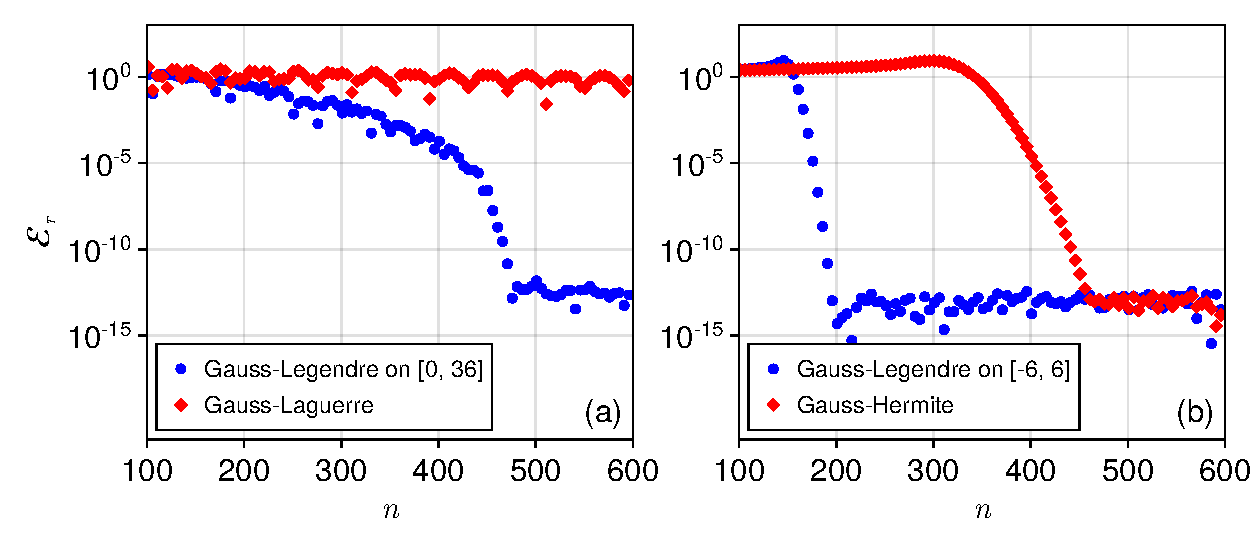
\includegraphics[width = \linewidth]{figs/integral_n.pdf}
    \caption{
        The relative error of numerical evaluation of integrals (a) Eq.~\eqref{eq:I1} via Gauss–Laguerre quadrature and (b) Eq.~\eqref{eq:I2} via Gauss–Hermite quadrature on infinite interval or Gauss-Legendre quadrature on truncated interval, respectively,~$n$ is the order of the quadrature.
    }
    \label{fig:Gauss_int}
\end{figure}

\begin{figure}[htbp]
    \centering
    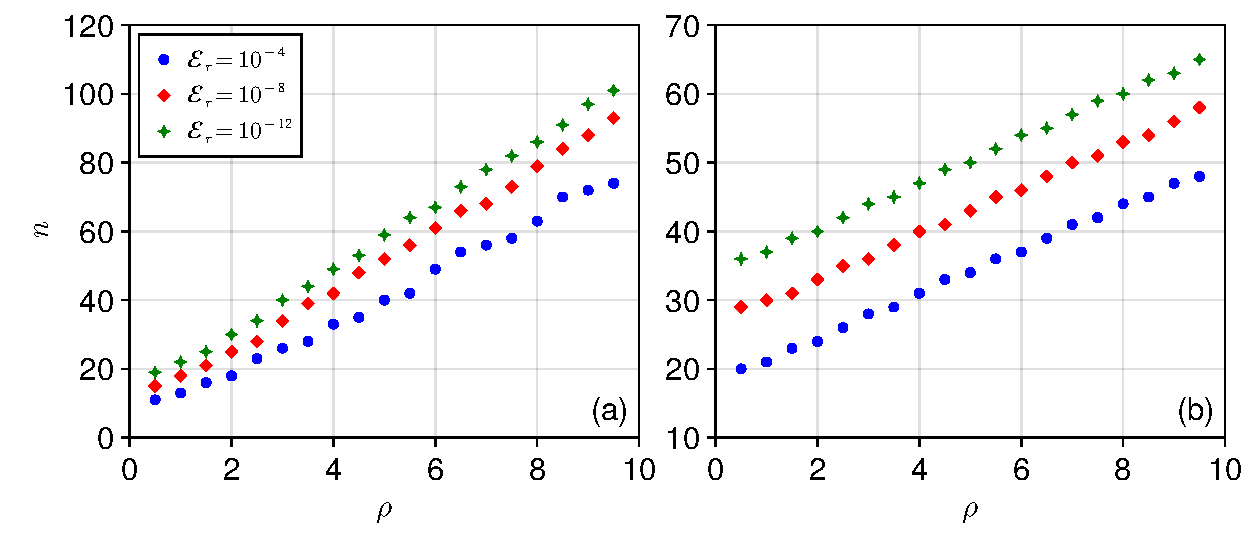
\includegraphics[width = \linewidth]{figs/integral_r.pdf}
    \caption{
    Order of quadrature~$n$, needed to numerically evaluate the integrals (a) Eq.~\eqref{eq:I1} and (b) Eq.~\eqref{eq:I2} to reach the given relative accuracy~$\mathcal{E}_r$ using the Gauss-Legendre quadrature on truncated interval~$[0, k_{c1}]$ and~$[-k_{c2}, k_{c2}]$, respectively.
    }
    \label{fig:Gauss_int_n}
\end{figure}

Then we consider the long-range part~$U_\ell$.
As the long range interaction  energy $U_\ell$ reads
\begin{align*} 
U_\ell&=\frac{1}{4  L_xL_y}\sum_{i,j=1}^N q_iq_j\Bigg({\Abs{z_i-z_j}} +\\&~~~~+  \sum_{\V{h}\in\fK^2,\V{h}\neq\vzero} \frac{ \exp{(\mathrm{i} \V{h} \cdot \V{\rho}_{ij})}}{k\left(1-\gamma_{\mrm{u}}\gamma_{\mrm{d}}\exp(-2hH)\right)}\left[\sum_{p=1}^4\Gamma_p\exp(-ha_p(z_i;z_j))\right] \exp\left(-\frac{h^2}{4\alpha}\right)\Bigg)\;,
\end{align*}
and we endeavor to  reduce the $\fO(N^2)$ complexity to linear scaling by incorporating the idea of random batch sampling in combination with the summation-via-sorting technique that has been discussed in Chapter~\ref{chp_soewald2d}.

%Firstly, we shall deal with the summation over $i$ and $j$, i.e., $\sum_{i,j=1}^N$. 
We observe that the four components in the following summation read
\begin{align*}
     &\sum_{p=1}^4\Gamma_p\exp(-ha_p(z_i;z_j))\\  
     =&\exp(- h \Abs{z_i-z_j})+\gamma_{\mrm{d}}\exp(-h(z_i+z_j))\\
     &+\gamma_{\mrm{u}}\exp(-h(2H-z_i-z_j)) +\gamma_{\mrm{u}}\gamma_{\mrm{d}}\exp(-h(2H-\Abs{z_i-z_j}))\;.
\end{align*}
%%%%%%%%%%%%%%%%%%%%%%%%%%%%%%%%%%%%%%%%%%%%%%%%%%%%%%%%%%
To facilitate the computation, we define auxiliary functions $\beta_{1:4}(h)$ as 
\begin{align*}
    \beta_1(\V{h})&:= \frac{1}{4  L_xL_yh\left(1-\gamma_{\mrm{u}}\gamma_{\mrm{d}}\exp(-2hH)\right)} \;,\\
    \beta_2(\V{h})&:= \frac{\gamma_{\mrm{d}}}{4  L_xL_yh\left(1-\gamma_{\mrm{u}}\gamma_{\mrm{d}}\exp(-2hH)\right)} \;,\\
    \beta_3(\V{h})&:= \frac{\gamma_{\mrm{u}}\exp(-2hH)}{4  L_xL_yh\left(1-\gamma_{\mrm{u}}\gamma_{\mrm{d}}\exp(-2hH)\right)}\;,\\
    \beta_4(\V{h})&:= \frac{\gamma_{\mrm{u}}\gamma_{\mrm{d}}\exp(-2hH)}{4  L_xL_yh\left(1-\gamma_{\mrm{u}}\gamma_{\mrm{d}}\exp(-2hH)\right)}\;,
\end{align*}
and another set of auxiliary functions   $S_{0:4}(k)$ as
%which allows us to express the summation over $i$ and $j$ in  $U_\ell$ as
\begin{align*} 
    S_0&:=\frac{1}{4  L_xL_y}\sum_{i,j=1}^Nq_iq_j {\Abs{z_i-z_j}}\;,\\
    S_1(\V{h})&:=\sum_{i,j=1}^Nq_iq_j  \exp{(\mathrm{i} \V{h} \cdot \V{\rho}_{ij})}\exp(-h\Abs{z_i-z_j})\;,\\
    S_2(\V{h})&:=\sum_{i,j=1}^Nq_iq_j  \exp{(\mathrm{i} \V{h} \cdot \V{\rho}_{ij})}\exp(-h(z_i+z_j))\;,\\
    S_3(\V{h})&:=\sum_{i,j=1}^Nq_iq_j  \exp{(\mathrm{i} \V{h} \cdot \V{\rho}_{ij})}\exp(h(z_i+z_j))\;,\\
    S_4(\V{h})&:=\sum_{i,j=1}^Nq_iq_j \exp{(\mathrm{i} \V{h} \cdot \V{\rho}_{ij})}\exp(h\Abs{z_i-z_j})\;.
\end{align*}
Consequently, the long-range interaction energy   $U_\ell$ reads
\begin{equation}\label{eq...text...Energy}
    U_\ell = S_0+ \sum_{\V{h}\in\fK^2,\V{h}\neq\vzero} \exp\left(-\frac{h^2}{4\alpha}\right)\sum_{p=1}^4S_p(\V{h}) \beta_p(\V{h})\;.
\end{equation}
and for simplicity, we denote hereafter in this paper that 
\begin{equation}\label{eq...text...phi}
    \phi(\V{h}):=\sum_{p=1}^4S_p(\V{h}) \beta_p(\V{h})\;,
\end{equation}
and on the basis of Eq. \eqref{eq...text...phi}, the   energy   $U_\ell$ can be simplified into 
\begin{equation} \label{eq...text...EnergywithPhi}
U_\ell =    S_0+ \sum_{\V{h}\in\fK^2,\V{h}\neq\vzero} \phi(\V{h})\exp\left(-\frac{h^2}{4\alpha}\right) \;,
\end{equation}
and the idea of random batch sampling is employed to efficiently evaluate the summation over   $\V{h}$, i.e., $\sum_{\V{h}\in\fK^2,\V{h}\neq\vzero}$. 
%However, prior to this step, we shall  introduce some alignment techniques to further enhance computational efficiency.
% \subsubsection{Part One: Pairwise summation}
It is easy to observe that  the  auxiliary functions  $S_2(\V{h})$ and $S_3(\V{h})$ are multiplicatively separable  in the sense that  they can be written into
\begin{align*}
S_2(\V{h})&=\sum_{i,j=1}^Nq_iq_j  \exp{(\mathrm{i} \V{h} \cdot \V{\rho}_{ij})}\exp(-h(z_i+z_j))\\
&=\left(\sum_{i=1}^Nq_i\exp{(\mathrm{i} \V{h} \cdot \V{\rho}_{i})}\exp(-hz_i)\right)\left(\sum_{j=1}^Nq_j\exp{(-\mathrm{i} \V{h} \cdot \V{\rho}_{j})}\exp(-hz_j)\right)\;,\\
S_3(\V{h})&=\sum_{i,j=1}^Nq_iq_j  \exp{(\mathrm{i} \V{h} \cdot \V{\rho}_{ij})}\exp(h(z_i+z_j))\\
&=\left(\sum_{i=1}^Nq_i  \exp{(\mathrm{i} \V{h} \cdot \V{\rho}_{i})}\exp(hz_i)\right)\left(\sum_{j=1}^Nq_j  \exp{(-\mathrm{i} \V{h} \cdot \V{\rho}_{j})}\exp(hz_j)\right)\;,
\end{align*}
such factorization significantly reduces computational complexity, as the direct evaluation of the double summation requires 
$\fO(N^2)$ operations, whereas the factorized form allows computation in only 
$\fO(N)$ steps.

However, the functions $S_0$,  $S_1(\V{h})$ and $S_4(\V{h})$  are non-multiplicatively separable due to the presence of the absolute difference term $\abs{z_i - z_j}$ which prevents direct factorization. Consequently, the strategy employed for 
$S_2(\V{h})$ and $S_3(\V{h})$ is no longer applicable. To achieve linear computational complexity in evaluating these terms,  some specialized alignment techniques must be introduced.

Firstly, we sort all $N$ particles according to their positions along the 
$z$-axis, ensuring the ordering
\begin{equation*}
   0 < z_1 < z_2 <  \cdots <  z_{N - 1}<z_N < H\;.
\end{equation*}
Since for all  $i$, $z_i \in (0, H)$ is uniformly bounded, hence  the strategies such as the bucket sorting~\cite{corwin2004sorting} can be applied, and the computational cost can be of order~$O(N \log{N})$ or even  of order~$O(N)$. 
Once all $N$ particles are sorted according to their positions along the $z$-axis, we observe that $S_0$ can be written into
\begin{align*}
    S_0 
    & = \sum_{i = 1}^N q_i \left( \sum_{j = 1}^{i }{q_j (z_i - z_j)} \right) \\
    & = 2 \sum_{i = 1}^N q_i \left( z_i \sum_{j = 1}^{i }q_j - \sum_{j = 1}^{i }z_j q_j  \right) \;.
\end{align*}
To efficiently compute this summation, we introduce two auxiliary sequences  $\left\{T_1(i)\right\}_{i=1}^N$ and $\left\{T_2(i)\right\}_{i=1}^N$, both of which  can be iteratively updated as follows:
\begin{align*}
    &T_1(1)=q_1,~~T_1(i+1)=T_1(i)+q_{i+1}\;,\\
    &T_2(1)=z_1q_1,~~T_2(i+1)=T_2(i)+z_{i+1}q_{i+1}\;.
\end{align*}
Using these auxiliary sequences, 
$S_0$ can be efficiently calculated as
\[
S_0= 2 \sum_{i = 1}^N q_i \left( z_iT_1(i)-T_2(i)\right)\;,
\]
which requires only 
$4N$ operations, significantly reducing computational complexity in comparison with the naive summation.

A similar strategy~\cite{jiang2021approximating, gan2024fast} can also be applied to the evaluation of $S_1(\V{h})$ and $S_4(\V{h})$. For $S_1(\V{h})$, we obtain that 
\begin{align*}
S_1(\V{h})&=\sum_{i,j=1}^Nq_iq_j  \exp{(\mathrm{i} \V{h} \cdot \V{\rho}_{ij})}\exp(-h\Abs{z_i-z_j})\\
&=-\sum_{i=1}^Nq_i^2+\sum_{i=1}^N \sum_{j=1}^iq_iq_j  \exp{(\mathrm{i} \V{h} \cdot \V{\rho}_{ij})}\exp(-h(z_i-z_j))\\
&~~+\sum_{i=1}^N \sum_{j=i}^Nq_iq_j  \exp{(\mathrm{i} \V{h} \cdot \V{\rho}_{ij})}\exp(-h(z_j-z_i))\\
&= -\sum_{i=1}^Nq_i^2+\sum_{i=1}^N q_i\exp{(\mathrm{i} \V{h} \cdot \V{\rho}_{i})}\exp(-hz_i)\sum_{j=1}^iq_j\exp{(-\mathrm{i} \V{h} \cdot \V{\rho}_{j})}\exp(hz_j)\\
&~~+\sum_{i=1}^N q_i\exp{(\mathrm{i} \V{h} \cdot \V{\rho}_{i})}\exp(hz_i)\sum_{j=i}^Nq_j\exp{(-\mathrm{i} \V{h} \cdot \V{\rho}_{j})}\exp(-hz_j)\;,
\end{align*}
 we introduce another two auxiliary sequences  $\left\{T_3(i)\right\}_{i=1}^N$ and $\left\{T_4(i)\right\}_{i=1}^N$, and it is noteworthy that $\left\{T_3(i)\right\}_{i=1}^N$ is  constructed through forward iteration, whereas  $\left\{T_4(i)\right\}_{i=1}^N$   is generated through backward iteration:

\begin{align*}
    &T_3(1)=q_1\exp{(-\mathrm{i} \V{h} \cdot \V{\rho}_{1})}\exp(hz_1)\;,\\
    &T_3(i+1)=T_3(i)+q_{i+1}\exp{(-\mathrm{i} \V{h} \cdot \V{\rho}_{i+1})}\exp(hz_{i+1})\;,\\
    &T_4(N)=q_N\exp{(-\mathrm{i} \V{h} \cdot \V{\rho}_{N})}\exp(-hz_N)\;,\\
    &T_4(i-1)=T_4(i)+q_{i-1}\exp{(-\mathrm{i} \V{h} \cdot \V{\rho}_{i-1})}\exp(-hz_{i-1})\;,
\end{align*}
and
$S_1(\V{h})$ can be efficiently calculated as
\[
S_1(\V{h})= -\sum_{i=1}^Nq_i^2+ \sum_{i=1}^N q_i\exp{(\mathrm{i} \V{h} \cdot \V{\rho}_{i})}\left[\exp(-hz_i)T_3(i)+\exp(hz_i)T_4(i)\right]\;.
\]
As for $S_4(\V{h})$, we shall follow the same routine:
\begin{align*}
S_4(\V{h})&=\sum_{i,j=1}^Nq_iq_j  \exp{(\mathrm{i} \V{h} \cdot \V{\rho}_{ij})}\exp(-h\Abs{z_i-z_j})\\
&=-\sum_{i=1}^Nq_i^2+\sum_{i=1}^N \sum_{j=1}^iq_iq_j  \exp{(\mathrm{i} \V{h} \cdot \V{\rho}_{ij})}\exp(h(z_i-z_j))\\
&~~+\sum_{i=1}^N \sum_{j=i}^Nq_iq_j  \exp{(\mathrm{i} \V{h} \cdot \V{\rho}_{ij})}\exp(h(z_j-z_i))\\
&= -\sum_{i=1}^Nq_i^2+\sum_{i=1}^N q_i\exp{(\mathrm{i} \V{h} \cdot \V{\rho}_{i})}\exp(hz_i)\sum_{j=1}^iq_j\exp{(-\mathrm{i} \V{h} \cdot \V{\rho}_{j})}\exp(-hz_j)\\
&~~+\sum_{i=1}^N q_i\exp{(\mathrm{i} \V{h} \cdot \V{\rho}_{i})}\exp(-hz_i)\sum_{j=i}^Nq_j\exp{(-\mathrm{i} \V{h} \cdot \V{\rho}_{j})}\exp(hz_j)\;,
\end{align*}
and we introduce another two auxiliary sequences  $\left\{T_5(i)\right\}_{i=1}^N$ and $\left\{T_6(i)\right\}_{i=1}^N$, and it is noteworthy that $\left\{T_5(i)\right\}_{i=1}^N$ is  constructed through forward iteration, whereas  $\left\{T_6(i)\right\}_{i=1}^N$   is generated through backward iteration:

\begin{align*}
    &T_5(1)=q_1\exp{(-\mathrm{i} \V{h} \cdot \V{\rho}_{1})}\exp(-hz_1)\;,\\
    &T_5(i+1)=T_5(i)+q_{i+1}\exp{(-\mathrm{i} \V{h} \cdot \V{\rho}_{i+1})}\exp(-hz_{i+1})\;,\\
    &T_6(N)=q_N\exp{(-\mathrm{i} \V{h} \cdot \V{\rho}_{N})}\exp(hz_N)\;,\\
    &T_6(i-1)=T_6(i)+q_{i-1}\exp{(-\mathrm{i} \V{h} \cdot \V{\rho}_{i-1})}\exp(hz_{i-1})\;,
\end{align*}
and $S_4(\V{h})$ can be written as
\[
S_4(\V{h})= -\sum_{i=1}^Nq_i^2+ \sum_{i=1}^N q_i\exp{(\mathrm{i} \V{h} \cdot \V{\rho}_{i})}\left[\exp(hz_i)T_5(i)+\exp(-hz_i)T_6(i)\right]\;.
\]
To sum up, given fixed frequency $\V{h}^\ast$, it only takes  linear complexity to evaluate $S_0$ and $\phi(\V{h}^\ast)$, and we proceed to deal with the   summation over $\V{h}$. 
% \subsubsection{Part Two: Random Batch Importance Sampling}

% Then we introduce a stochastic algorithm designed to accelerate the Quasi-Ewald method in particle simulations, reducing the complexity to $O(N)$. 
% Unlike existing methods relying on either FFT or FMM-based techniques to reduce the complexity, our idea involves adopting mini-batch stochastic approximation over Fourier modes, with importance sampling for variance reduction. 
% More precisely, let us consider the Fourier sum over $\bm k \in \mathcal{K}^2$ for a given kernel $f(\bm{h})$,
% one can alternatively understand the Fourier sum as an expectation
% \begin{equation}
% 	\mu:=\sum_{\bm{h}\in\mathcal{K}^2}\frac{f(\bm{h})}{g(\bm{h})}g(\bm{h})=\mathbb{E}_{\bm k\sim g(\bm{h})}\left[\frac{f(\bm{h})}{g(\bm{h})}\right],
% \end{equation}
% where $g(\bm{h})$ is a probability measure defined on the lattice $\bm k \in \mathcal{K}^2$ and the expectation~$\mathbb{E}_{\bm k\sim g(\bm{h})}$ is taken with respect to the probability measure.
% Instead of calculating the summation directly or using FFT, a mini-batch of Fourier modes (with batch size $P$) sampled from $g(\bm{h})$ are employed to estimate the expectation, resulting in an efficient stochastic algorithm.

% It is worth noting that the random mini-batch strategy originated from stochastic gradient descent in machine learning and was first introduced in the study of interacting particle systems by Jin et al.~\cite{jin2020random}, called the random batch method. 
Observe that the long-range interaction energy $U_\ell$ can be represented as
\[
U_\ell =   S_0+ \sum_{\V{h}\in\fK^2,\V{h}\neq\vzero}\phi(\V{h}) \exp\left(-\frac{h^2}{4\alpha}\right) \;,
\]
we define 
\begin{equation}\label{eq::U_l0_Ulk}
    U_\ell^{\vzero} := S_0,\quad\text{and}\quad U_\ell^{\V{h}\neq \vzero} :=\sum_{\V{h}\in\fK^2,\V{h}\neq\vzero}\phi(\V{h}) \exp\left(-\frac{h^2}{4\alpha}\right) \;,
\end{equation}
then $U_\ell$ can be written into the sum of these two components
\[
U_\ell= U_\ell^{\vzero}+U_\ell^{\V{h}\neq \vzero}\;,
\]
Since 
$ U_\ell^{\vzero}$
can be computed with linear complexity, we focus on the efficient evaluation of 
$U_\ell^{\V{h}\neq \vzero}$, for which the idea of random batch is employed.
Based on the above expression, we find a Gaussian decay factor in $U_\ell^{\V{h}\neq \vzero}$ explicitly, which can be normalized for the  purpose of importance sampling, so that again we apply the idea of random batch sampling taking
\begin{equation}\label{eq::hk}
	g(\bm{h}) := \frac{1}{S} \exp\left(-\frac{h^2}{4\alpha}\right)\;, %\quad H := \sum_{\bm{h}\neq\bm{0}}e^{-h^2/(4\alpha^2)},
\end{equation}
where \[S:= \sum_{\V{h}\in\fK^2,\V{h}\neq\vzero}\exp\left(-\frac{h^2}{4\alpha}\right)\;,\] serves as a normalization factor.
% By application of the Poisson summation formula, $H$ can be computed as follows
%
% \begin{align*}
%   H+1&=  \sum_{\V{h}\in\fK^2}\exp\left(-\frac{h^2}{4\alpha}\right)\;,\\
%   \sum_{\V{h}\in\fK^2}\exp\left(-\frac{h^2}{4\alpha}\right)&= \frac{\alpha L_xL_y}{\pi}\sum_{m_x,m_y\in\mathbb{Z}}\exp\left({-\alpha\left(m_x^2L_x^2+m_y^2L_y^2\right)}\right)\;,
% \end{align*}
%
% hence
%
% \begin{equation}\label{eq::Happ}
% 	H=-1+\frac{\alpha L_xL_y}{\pi}\sum_{m_x,m_y\in\mathbb{Z}}\exp\left({-\alpha\left(m_x^2L_x^2+m_y^2L_y^2\right)}\right)\;,
% \end{equation}
%
Using the Metropolis algorithm~\cite{metropolis1953equation}, a random mini-batch of frequencies $\{\bm{h}_{\eta}\}_{\eta=1}^P$ is sampled, where~$P$ is the batch size, and $U_\ell$ can be approximated as 
\begin{equation}\label{eq::RBapp}
 U_\ell^{\V{h}\neq \vzero} \approx U_{l,\ast}^{\V{h}\neq \vzero}  :=   \frac{S}{P}\sum_{\eta=1}^P \phi(\V{h}_{\eta})=  \frac{S}{P}\sum_{\eta=1}^P \sum_{q=1}^4S_q(\V{h}_{\eta})h_q(\V{h}_{\eta})\;,
\end{equation} 
and the corresponding estimator of the force in Fourier space is given by
\begin{equation}
	 \bm{F}_{l,i}\approx\bm{F}_{l,i}^*=-  \grad_{\V{r}_i} U_\ell^{\vzero}- \grad_{\V{r}_i} U_{l,\ast}^{\V{h}\neq \vzero}\;,
 \end{equation}
Finally, combining all these strategies, we state our Quasi-Ewald method for calculating the electrostatic energy and forces in molecular dynamics simulations, see Algorithm~\ref{alg:rbqe}.
\begin{algorithm}[ht] 
\caption{The Quasi-Ewald method}
\begin{algorithmic}[1]
    \State \textbf{Input}:  Initialize the size of the simulation box $(L_x,L_y, H)$, as well as the positions, velocities, and charges of all particles. Choose a precision requirement $\varepsilon$ as well as batch size $P$.
    \State \textbf{Precomputation}:  Determine Ewald splitting parameters $\alpha$. Generate real space cutoff by $r_c$.
    \Procedure\text{Quasi-Ewald}{}       
        \State Draw $P$ frequencies $\{\bm{h}_{\eta}\}_{\eta=1}^{P}$ using the Metropolis algorithm;
        \State Sort all the particles according to their $z$ coordinates, such that $z_1 < z_2 < \cdots < z_N$;
        \State Compute unbiased Fourier space energy $U_{l, *}^{\bm{h}\neq\bm{0}}$ by importance sampling Eq.~\eqref{eq::RBapp};
        \State Compute zero-frequency part $U_{l}^{\bm{0}}$ according to Eq.~\eqref{eq::U_l0_Ulk}.
        % \State Compute $U_{\text{self}}$ and $U_{\text{p-s}}$ via Eqs.~\eqref{eq::self} and \eqref{eq:spectial}, respectively.
        \State Compute~$U_{s}^{*}$ by direct truncation in real space according to Eq.~\eqref{eq::U_s_truncated} with cutoff $r_c$. %\Comment{short-range part}
        \State Compute $U^{*} = U_{s, *} + U_{l}^{\bm{0}} + U_{l, *}^{\bm{h}\neq\bm{0}}$.
        \State Compute forces $\bm{F}_{i}^{*}$ via a similar procedure as that of $U^{*}$.
    \EndProcedure

    \State \textbf{Output}: Unbiased estimation of electrostatic energy $U^{*}$ and forces $\bm{F}_{l,i}^{*}$.
\end{algorithmic}\label{alg:rbqe}
\end{algorithm}
% \begin{algorithm}
% \caption{The Quasi-Ewald method}
% \label{alg:rbqe}
% \begin{algorithmic}
% \STATE{Choose~$\alpha$, the cutoff in real space~$\rho_c$, truncation point of the integrals~$k_c$, the number of points for the Gaussian quadrature~$n$, the batch size~$p$ and~$d t$.}
% \STATE{Randomly initialize the positions and velocities of charges~$\V{r}_i$ and~$\V{v}_i$ for~$1 \leq i \leq N$.}
% \STATE{Sample sufficient number of~$\V{h}$ according to distribution $\exp{(-h^2 / (4 \alpha))} / H$, $k \neq 0$ to from a set~$\mathcal{K}$.}
% \FOR{step in 1 : Step}
%     \STATE{Find neighbors of each particle using cell list, then compute the short range parts of the Coulomb interaction by Eq.~\eqref{eq:F_short}, with a complexity of~$O(nN)$.}
%     \STATE{Sort all particles up in the $z$ direction, and randomly take~$p$ frequencies from the set~$\mathcal{K}$, and then estimate the long range interaction using Eq.~\eqref{eq:F_l_rbe}, with a complexity of~$O(pN)$.}
%     \STATE{Integrate Newton's equations~\eqref{eq:NewtonEquation} for time~$d t$ via velocity-Verlet method and some appropriate thermostat, with a complexity of~$O(N)$.}
% \ENDFOR
% \end{algorithmic}
% \end{algorithm}

\subsection{Consistency and variance analysis}
In this section, we provide theoretical analysis for the Quasi-Ewald method. We start with considering the fluctuations, i.e., the stochastic error introduced by the importance sampling at each time step.
The fluctuations for the Fourier space components of   the force acting on the $i$th particle are defined as follows 
\begin{equation}\label{eq::xichi}
%	\Xi :=U_{l,\ast}^{\V{h}\neq \vzero}-U_\ell^{\V{h}\neq \vzero},\quad\text{and}\quad
    \V{\chi}_{i} :=\vF_{l,i}^*-\vF_{l,i}=\grad_{\V{r}_i} U_{l,\ast}^{\V{h}\neq \vzero}-\grad_{\V{r}_i} U_{l}^{\V{h}\neq \vzero}\;.
\end{equation}
Proposition~\ref{prop:unbaised} is obtained directly by the definition of the importance sampling.
\begin{prop}\label{prop:unbaised}
	  $\vF_{l,i}^*$ is a  unbiased estimator, i.e.,  $\mathbb{E} \V{\chi}_{i} = \bm 0$, and its variance  can be expressed by
% \begin{align*}
% 		\mathbb{E}\Xi^2&=\frac{S}{P}\sum_{\bm{h}_1\in\fK^2, \bm{h}_1\neq \vzero}\exp\left(-\frac{\Norm{\V{h}_1}^2}{4\alpha}\right)\Abs{\phi(\V{h}_1)-\frac{1}{H} \sum_{\bm{h}_2\in\fK^2, \bm{h}_2\neq \vzero}\phi(\V{h}_2)\exp\left(-\frac{\Norm{\V{h}_2}^2}{4\alpha}\right)}^2\;,
%         % \\
%         % \Bigg|\sum_{q=1}^4S_q(\V{h}_{1})h_q(\V{h}_{1})\\
%         % &~~~~~~~~~~~~~~~~~~~~~~~~~~~~~~~~~-\frac{1}{H} \sum_{\bm{h}_2\neq \vzero}\exp\left(-\frac{\Norm{\V{h}_2}^2}{4\alpha}\right)\sum_{q=1}^4S_q(\V{h}_{2})h_q(\V{h}_{2}) \Bigg|^2\;,
% \end{align*}
% 	and
\begin{align*}
		\mathbb{E}\Norm{\V{\chi}_{i}}^2&=\frac{S}{P}\sum_{\bm{h}_1\in\fK^2, \bm{h}_1\neq \vzero}\exp\left(-\frac{\Norm{\V{h}_1}^2}{4\alpha}\right)\Bigg|\Bigg|\nabla_{\bm{r}_i}\phi(\V{h}_1)\\
        &~~~~~~~~~~~~~~~~~~~~~~~~~~~~~~~~~~~~~-\frac{1}{H} \sum_{\bm{h}_2\in\fK^2, \bm{h}_2\neq \vzero}\nabla_{\bm{r}_i}\phi(\V{h}_2)\exp\left(-\frac{\Norm{\V{h}_2}^2}{4\alpha}\right)\Bigg|\Bigg|^2\;.
\end{align*}
\end{prop}
% Furthermore, under the Debye-H$\ddot{\text{u}}$ckel approximation~\cite{levin2002electrostatic}, we have  the following~Lemma~\ref{lem::upper_bound_phiRB}, whose proof can be found in Appendix G in~\cite{gan2024fast}.
% \begin{lem} \label{lem::upper_bound_phiRB}
%   Under the assumption of the DH theory, given function of the form 
%     \begin{equation}
%        \mathscr{G}(\V{r}_i)=\sum_{j\neq i}q _i q_{j}\exp{(\mathrm{i} \V{h} \cdot \V{\rho}_{ij})}f(z_{ij}),
%     \end{equation}
%  where $\abs{f(z_{ij})}$ is bounded by  a constant $C_f$ independent of $z_{ij}$, then function $ \mathscr{G}(\V{r}_i)$ is bounded above by
%     \begin{equation}
%          \mathscr{G}(\V{r}_i)\leq q_i  C_f\lambda_{D}^2\;,
%     \end{equation}
%     where~$\lambda_{D}$  represents the Debye length.
% 	% Under the assumption of the DH theory, $|\phi(\bm{h})|$ and $\Norm{\nabla_{\bm{r}_i}\phi(\bm{h})}$ have their respective upper bounds
% 	% \begin{equation}
% 	% 	\abs{ \widetilde{\varphi}^{\emph{RB}}(\bm{h})}\leq\frac{2\sqrt{\pi}\lambda_D^2 Q}{L_xL_y k}\left(\sqrt{\pi}+\frac{\alpha \varepsilon}{k}\right),
% 	% 	\quad
% 	% 	\abs{\nabla_{\bm{r}_{i}} \widetilde{\varphi}^{\emph{RB}}(\bm{h})}\leq  \frac{\pi \lambda_D^2 q_{i}^2}{L_xL_y}\left[3+\frac{\alpha}{\sqrt{\pi}}\left(1+\frac{2\sqrt{2}\varepsilon}{k}\right)\right], 
% 	% \end{equation}
% 	% where $\lambda_{D}$ represents the Debye length
% \end{lem}


Finally, we introduce the following Theorem~\ref{thm:unbaised} for the boundedness and convergence in the fluctuations originated from the random batch approximation.
\begin{thm}\label{thm:unbaised}
	Under the assumption of the DH theory, the variance of the estimators of forces have closed upper bounds
	\begin{equation}
		  \mathbb{E}\Norm{\V{\chi}_{i}}^2\leq\frac{ S^2q_i^2\lambda_{D}^4}{2P ^2 L_x^2L_y^2}\left( \frac{1+\Abs{\gamma_{\mrm{u}}}+\Abs{\gamma_{\mrm{d}}}+\Abs{\gamma_{\mrm{u}}\gamma_{\mrm{d}}}}{1-\max\{0,\gamma_{\mrm{u}}\gamma_{\mrm{d}}\}}\right)^2\;,
	\end{equation}
     where~$\lambda_{D}$  represents the Debye length.
\end{thm}
\begin{proof}
We observe that 
\begin{align*}
 \nabla_{\bm{r}_i}\phi(\V{h})&=   \sum_{q=1}^4 \nabla_{\bm{r}_i}\left\{S_q(\V{h})\right\}h_q(\V{h})\;,
\end{align*}
thus we have,
%
% \begin{align*}
%  \nabla_{\bm{r}_i} S_q(\V{h})&= \begin{pmatrix} \nabla_{\vrho_i}S_q(\V{h})\\
% \partial_{z_i}S_q(\V{h}) \end{pmatrix}   = \begin{pmatrix} \mathrm{i} \V{h}S_q(\V{h})\\
% \pm k S_q(\V{h}) \end{pmatrix} =\begin{pmatrix} \mathrm{i} \V{h} \\
% \pm k  \end{pmatrix}S_q(\V{h})\;,
% \end{align*}
%
\begin{align*}
 \nabla_{\bm{r}_i} S_1(\V{h})&=\sum_{j,j\neq i}q_iq_j   \begin{pmatrix} \mathrm{i} \V{h} \\
 \pm h  \end{pmatrix}\exp{(\mathrm{i} \V{h} \cdot \V{\rho}_{ij})}\exp(-h\Abs{z_i-z_j})\;,\\
 \nabla_{\bm{r}_i} S_2(\V{h})&=\sum_{j,j\neq i}q_iq_j   \begin{pmatrix} \mathrm{i} \V{h} \\
 -h  \end{pmatrix}\exp{(\mathrm{i} \V{h} \cdot \V{\rho}_{ij})}\exp(-h(z_i+z_j))\;,\\
  \nabla_{\bm{r}_i} S_3(\V{h})&=\sum_{j,j\neq i}q_iq_j   \begin{pmatrix} \mathrm{i} \V{h} \\
 h  \end{pmatrix}\exp{(\mathrm{i} \V{h} \cdot \V{\rho}_{ij})}\exp(h(z_i+z_j))\;,\\
 \nabla_{\bm{r}_i} S_4(\V{h})&=\sum_{j,j\neq i}q_iq_j   \begin{pmatrix} \mathrm{i} \V{h} \\
 \pm h  \end{pmatrix}\exp{(\mathrm{i} \V{h} \cdot \V{\rho}_{ij})}\exp(h\Abs{z_i-z_j})\;,\\
\end{align*}
and  the choice of $+$ or $-$ depends on the choice of particle. Consequently, $\grad_{\V{r}_i} \phi(\V{h})$ takes the form
\begin{align*}
  \grad_{\V{r}_i} \phi(\V{h})  &=\sum_{j,j\neq i}q_iq_j  \exp{(\mathrm{i} \V{h} \cdot \V{\rho}_{ij})} \begin{pmatrix} \mathrm{i} \V{h} \\
 \pm h  \end{pmatrix}g(z_{ij})\;,
\end{align*}
where the estimates on $g(z_{ij})$ reads
\begin{align*}
  \Abs{g(z_{ij})  }&\leq  \frac{1+\Abs{\gamma_{\mrm{u}}}+\Abs{\gamma_{\mrm{d}}}+\Abs{\gamma_{\mrm{u}}\gamma_{\mrm{d}}}}{4  L_xL_y h \left(1-\max\{0,\gamma_{\mrm{u}}\gamma_{\mrm{d}}\}\right)}\;,
\end{align*}
on the basis of Lemma \ref{lem::upper_bound_phiRB}, the upper bound of~$\abs{\grad_{\V{r}_i} \phi(\V{h})}$ can be estimated as follows 
\begin{equation}
  \Norm{\nabla_{\bm{r}_i}\phi(\V{h})}\leq \frac{q_i\lambda_{D}^2}{2  L_xL_y}    \frac{1+\Abs{\gamma_{\mrm{u}}}+\Abs{\gamma_{\mrm{d}}}+\Abs{\gamma_{\mrm{u}}\gamma_{\mrm{d}}}}{1-\max\{0,\gamma_{\mrm{u}}\gamma_{\mrm{d}}\}}\;.
\end{equation}
Finally,  variance of force on the $i$-th particle is bounded above by
\begin{align*}
   	\mathbb{E}\Norm{\V{\chi}_{i}}^2&\leq   \frac{2S}{P}\sum_{\bm{h}_1\in\fK^2, \bm{h}_1\neq \vzero}\exp\left(-\frac{\Norm{\V{h}_1}^2}{4\alpha}\right)\Norm{\nabla_{\bm{r}_i}\phi(\V{h}_1)}^2\\
    &\leq  \frac{2S^2}{P}\left(\frac{q_i\lambda_{D}^2}{2  L_xL_y}    \frac{1+\Abs{\gamma_{\mrm{u}}}+\Abs{\gamma_{\mrm{d}}}+\Abs{\gamma_{\mrm{u}}\gamma_{\mrm{d}}}}{1-\max\{0,\gamma_{\mrm{u}}\gamma_{\mrm{d}}\}}\right)^2\\
    &= \frac{ S^2q_i^2\lambda_{D}^4}{2P ^2 L_x^2L_y^2}\left( \frac{1+\Abs{\gamma_{\mrm{u}}}+\Abs{\gamma_{\mrm{d}}}+\Abs{\gamma_{\mrm{u}}\gamma_{\mrm{d}}}}{1-\max\{0,\gamma_{\mrm{u}}\gamma_{\mrm{d}}\}}\right)^2\;.
\end{align*}
\end{proof}
We remark that $S \sim L_xL_y$, then $	\mathbb{E}\Norm{\V{\chi}_{i}}^2=\fO\left(\frac{1}{P}\right)$ and independent of the particle number $N$.
Theorem~\ref{thm:unbaised} has demonstrated that the variance of force scales as $\fO\left(\frac{1}{P}\right)$, unaffected by the growth of the system size $N$, provided the same   Debye length $\lambda_{D}$. 
This is crucial for its practical usage in MD simulations, where the dynamical evolution typically relies on force calculations rather than energy. 
We proceed to demonstrate  
%some analysis for the strong convergence of the random batch MD, which further supports this observation. The following result indicates 
that random mini-batch methods can be valid for capturing the finite time dynamics
(we take the Langevin thermostat for illustration). Before that, we shall introduce  some additional notations.
Let $d t$ be the discretized time step, and $\bm{r}_i$, $m_i$, and $\bm{p}_i$ represent the position, mass, and momentum of the $i$th particle, respectively. 
\begin{thm}(Strong convergence)
Let $(\bm{r}_i, \bm{v}_i)$ be the solutions to
\[
\begin{split}
&d\bm{r}_i=\bm{v}_i\,d t\;,\\
&m_i d\bm{v}_i=\left[\bm{F}_i-\gamma \bm{v}_i\right]\,d t+\sqrt{\frac{2\gamma}{\beta}}d \bm{W}_i\;,
\end{split}
\]
where $\{\bm{W}_i\}_{i=1}^N$ are i.i.d. Wiener processes. Let $(\widetilde{\bm{r}}_i, \widetilde{\bm{v}}_i)$ be the solutions to
\[
\begin{split}
&d \widetilde{\bm{r}}_i=\widetilde{\bm{v}}_i\,d t\;,\\
&m_i d\widetilde{\bm{v}}_i=\left[\bm{F}_i +\bm{\chi}_i-\gamma \widetilde{\bm{v}}_i\right]\,d t+\sqrt{\frac{2\gamma}{\beta}}d \bm{W}_i\;,
\end{split}
\]
with the same initial values as $(\bm{r}_i, \bm{v}_i)$. Suppose that the masses $m_i$'s are bounded uniformly from above and below.
If the forces $\bm{F}_i$ are bounded and Lipschitz and $\Exp \bm{\chi}_i=0$, then for any $T>0$, there exists $C(T)>0$ such that
\[
\Exp\left[\frac{1}{N}\sum_i (\Norm{\bm{r}_i-\widetilde{\bm{r}}_i}^2
+\Norm{\bm{v}_i-\widetilde{\bm{v}}_i}^2) \right] \leq C(T)\sqrt{\Lambda dt}\;,
\]
where $\Lambda$ is an upper bound for $\max_i  \Exp\Norm{\bm{\chi}_i}^2$.
\end{thm}

Proofs for similar interacting particle systems can be found in \cite{jin2021convergence,li2019stochastic,li2020random}, and thus, we do not include the proof for the claims here. Given the assumption that $\bm{F}_i$ is bounded and Lipschitz, the claims above are not directly applicable to our problem. Nevertheless, they provide valuable insights into the functioning of random batch methods.

According to the discussions above, QEM should be good for~$NVT$ simulations just like other random batch methods \cite{jin2020random, jin2021random}, since the error caused by sampling can be regarded as a type of thermal fluctuation, and can be properly canceled via coupling the system with a heat bath by applying proper thermostats.

Finally, the optimal time complexity of QEM is given by
\begin{align}
    C_s & \propto \pi r_c^2 \frac{N^2}{L_x L_y}\;,\\
    C_\ell & \propto N P\;,
\end{align}
where~$C_s$ and~$C_\ell$ are the cost of computing the short range and the long range part, respectively.
Since the decaying rate of the energy is given by~$\Delta U_s \propto (\alpha r_c^3)^{-1}$, the cutoff can be chosen as
\begin{equation}
    r_c = (10^{-E} \alpha)^{-\frac{1}{3}}\;,
\end{equation}
where~$E$ represents the upper bound of the truncation error of the pairwise short range interaction.
Then by taking
\begin{equation}\label{eq:alphs-select}
    \alpha = \left(\frac{N}{L_x L_y} \right)^{1.5} = {\varrho}^{1.5}\;,
\end{equation}
where~$\varrho$ represents the surface density.
The cost of the short range interaction is given by
\begin{equation}
    C_s \propto  N\;.
\end{equation}
In this way, total cost of the QEM will be of~$O(N)$.

% \begin{rmk}
%     With the~$\alpha$ selected according to Eq.~\eqref{eq:alphs-select}, the variance of force can be estimated as
%     \begin{equation}
%         \mathbb{E} {\abs{\V{\chi}}_i}^2  \sim \frac{1}{p} \lambda_D^4 \varrho^{3}\;,
%     \end{equation}
%     which is irrelevant to number of particle as the size of the system increases with a fixed surface density.
% \end{rmk}

\subsection{QEM for negatively confined systems}

We now extend the QEM to negatively confined systems, where the dielectric permittivities of the upper and lower substrates are negative, resulting in~$\gamma_u \gamma_d > 1$. 
In these systems, the image charge method (ICM) produces a divergent series of image charges, making ICM-based approaches inapplicable.
As discussed in Remark~\ref{Remark...Nonzero+larger}, the key challenge for QEM arises from the divergence of the Green's function along the positive real axis, which causes the integral in the short-range interaction to become ill-posed.
Here, we demonstrate singularity subtraction techniques can effectively handle this divergence, allowing us to develop an efficient computational method for negatively confined systems.

According to Eq.~\eqref{eq::int_Gs}, the integral to be evaluated numerically can be simplified as
\begin{equation}\label{eq::int_I}
    I = \int_0^{\infty} \frac{J_0(b h) \exp{(- a h)}}{\exp{( - 2 H (h - k_0))} - 1} \mathrm{d}h\;,
\end{equation}
where~$a$,~$H$ and~$b$ are positive constants, $J_0$ is the zeroth order Bessel function of the first kind and~$k_0 = {\ln{(\gamma_u \gamma_d)}} / {2H}$ is a 1st order pole.

To avoid the divergence, we calculate the principle value by splitting the integrand into two parts, given by
\begin{equation}\label{eq::split}
    \begin{split}
        f_{1} &=  \frac{J_0(b h) e^{- a h} - J_0(b k_0) e^{- a k_0}}{e^{- 2 H (h - k_0)} - 1} - J_0(b k_0) e^{- a k_0} \;, \\
        f_{2} &= \frac{J_0(b k_0) e^{- a k_0 - 2 H (h - k_0)}}{e^{- 2 H (h - k_0)} - 1} \;,
    \end{split}
\end{equation}
which are smooth and singular, respectively.

\begin{figure}[ht]
    \centering
    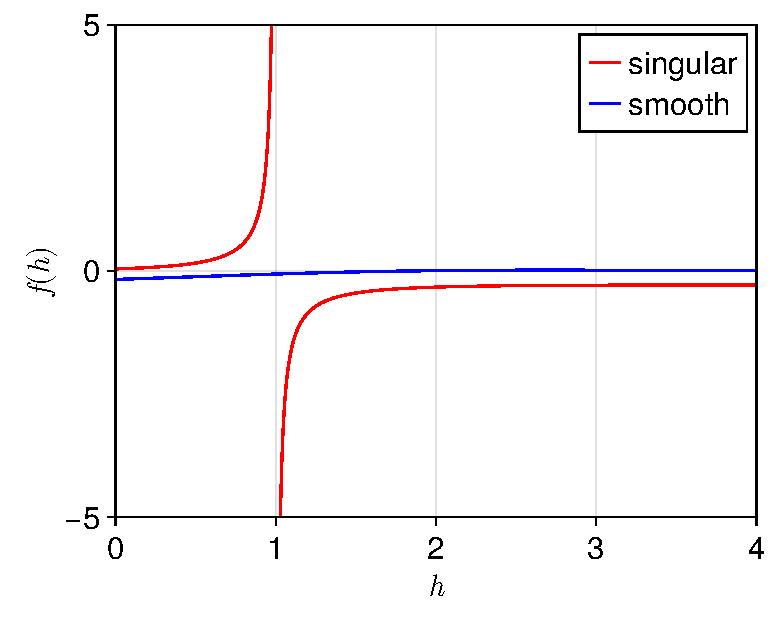
\includegraphics[width = 0.5\linewidth]{figs/fi.pdf}
    \caption{Illustration of the splitting of the integrand into smooth and singular parts as shown in Eq.~\eqref{eq::split}.}
    \label{fig:split}
\end{figure}

An example is shown in Fig.~\ref{fig:split}, where we take~$a = b = H = k_0 = 1$.
For the smooth part, when~$k \to k_0$, both the numerator and denominator tends to zero so that
\begin{equation}
    \lim_{h \to k_0} \frac{J_0(bh) e^{- a h} - J_0(bk_0) e^{- a k_0}}{e^{- 2 H (h - k_0)} - 1}  = \lim_{h \to k_0} \frac{ \partial {J_0(bh) e^{- a h}}}{ \partial {e^{- 2 H (h - k_0)}}}\;,
\end{equation}
which is a finite value, and the integrand is a smooth function at~$h = k_0$.
When~$h \gg 1$, the smooth part is rapidly decaying, 
\begin{equation}
    \abs{\frac{J_0(bh) e^{- a h} - J_0(bk_0) e^{- a k_0}}{e^{- 2 H (h - k_0)} - 1} + J_0(bk_0) e^{- a k_0} } \to \abs{J_0(bh) e^{- a h}}\;,
\end{equation}
so that the integral can be directly evaluated using the same method as in the previous section, given by
\begin{equation}
    \int_0^{\infty} \to \int_0^{k_f}\;,
\end{equation}
since we have shown that the integrand is rapidly decaying, the truncation error can be estimated by
\begin{equation}
    \delta I < \int_{k_f}^{\infty} \exp{(-a h)} dh < \frac{\exp{(-a h_f)}}{a}\;.
\end{equation}

Integral of the singular part can be calculated analytically, given by
\begin{equation}
    \begin{split}
        & \int_0^{\infty} \frac{J_0(bk_0) e^{- a k_0 - 2 H (h - k_0)}}{e^{- 2 H (h - k_0)} - 1} dh\\
        = & \frac{J_0(bk_0) e^{- a k_0}}{2H} \int_{0}^{\exp{(2 H k_0)}} \frac{1}{x - 1} dx\\
        = & \frac{J_0(bk_0) e^{- a k_0}}{2H} \ln{(\gamma_u \gamma_d - 1)}\;,
    \end{split}
\end{equation}
which is a finite value that can be easily calculated.

To verify the method above, we compared the result by the new approach shown above with a direct method given by
\begin{equation}
        I = \int_{0}^{2 k_0} \left[\frac{J_0(bh)e^{-ah}}{e^{-2H(h-k_0)} - 1} + \frac{J_0(bk_0)e^{-ak_0}}{2H(h - k_0)}\right] dh + \int_{2 k_0}^{\infty} \frac{J_0(bh)e^{-ah}}{e^{-2H(h-k_0)} - 1} dh\;.,\label{eq:direct}
\end{equation}
which directly subtracts the 1st order pole but take a high order of the Gaussian quadrature to reach high accuracy.

It is also shown that the integral converge much faster to the order of the quadrature.
We set~$a = b = k_0 = H = 1$, and $k_f = 10$,~$20$ and~$30$, the relative errors are shown in Fig.~\ref{fig:error} as functions of order of Gaussian quadrature, which shows that the error decay rapidly to desired accuracies.

\begin{figure}[htbp]
    \centering
    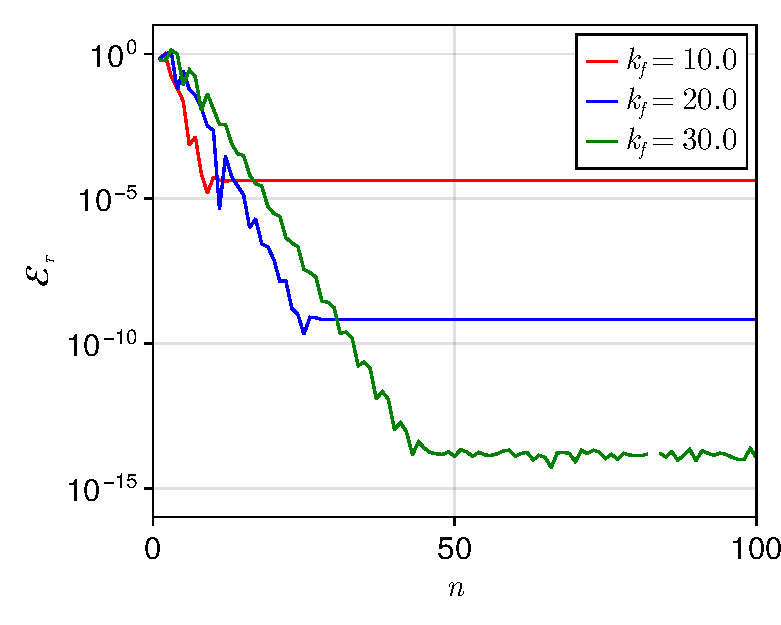
\includegraphics[width = 0.5\linewidth]{figs/int_convergence.pdf}
    \caption{Relative error of the numiercal evaluating Eq.~\eqref{eq::int_I} with $a = b = H = k_0 = 1$, as a function of cutoff~$k_f$ and order of the quadrature~$n$.}
    \label{fig:error}
\end{figure}

In summary, the singularity substraction tenchnique introduced above provides an efficient method for handling the singularity in the short-range interaction by splitting the integrand into smooth and singular parts that can be evaluated separately with high accuracy.
Thus, being combined with this technique, QEM enables the simulation of negatively confined Coulomb systems with high accuracy and efficiency.

\section{Numerical results}
\label{sec:result}

In this section, we validate the accuracy and efficiency of our proposed method by applying it to several typical scientific problems, some the results are compared with that of the previously proposed method, such as the Ewald2D method, the image charge method and the HSMA method.
The runtime of QEM in one of the typical scenario is also tested.
These examples indicate that the proposed method is effective and efficient.
% All calculations are performed in a Ubuntu system with AMD Ryzen Threadripper PRO 3995WX@2.2GHz, 1 CPU core.
Our software~\cite{QuasiEwald} is developed based on the Julia Programming Language~\cite{Julia-2017} and the open-source package \emph{CellListMap.jl}~\cite{celllistmap}.
The figures are generated by the open-source package \emph{Makie.jl}~\cite{DanischKrumbiegel2021}.

% \begin{rmk}
%     In this section, we focus on systems with positive permittivity, so that existing ICM-based methods can serve as reliable benchmarks. The numerical results for negatively confined systems will be presented in Section~\ref{sec::ssb}.
% \end{rmk}

\subsection{Interaction between charges}

In this subsection, we validate the accuracy and convergence of our method by calculating the electrostatic interaction energy and force between charged particles distributed in quasi-2D systems.
It is remarked that the importance sampling technique is not applied here.

We first consider the electrostatic interaction between a pair of charged particles, and the results are compared with that of the ICM-Ewald2D method.
We focused on two simple situations,~$\gamma_{d} = \gamma_{u} = \gamma = \pm 0.95$.
Size of the simulation box is set as~$(100, 100, 50)$, and the particle with charge~$+1$ is fixed at~$(50, 50, 1)$, while the other one with charge~$-1$ is moved along the $x$ axis or the $z$ axis.
For QEM, we set~$\alpha = 1.0$,~$n = 50$ and~$E = 4$.
The results are shown in Fig.~\ref{fig:E_xyz}, which indicates that QEM can accurately calculate the effects of the dielectric interface.

\begin{figure}[htb]
    \centering
    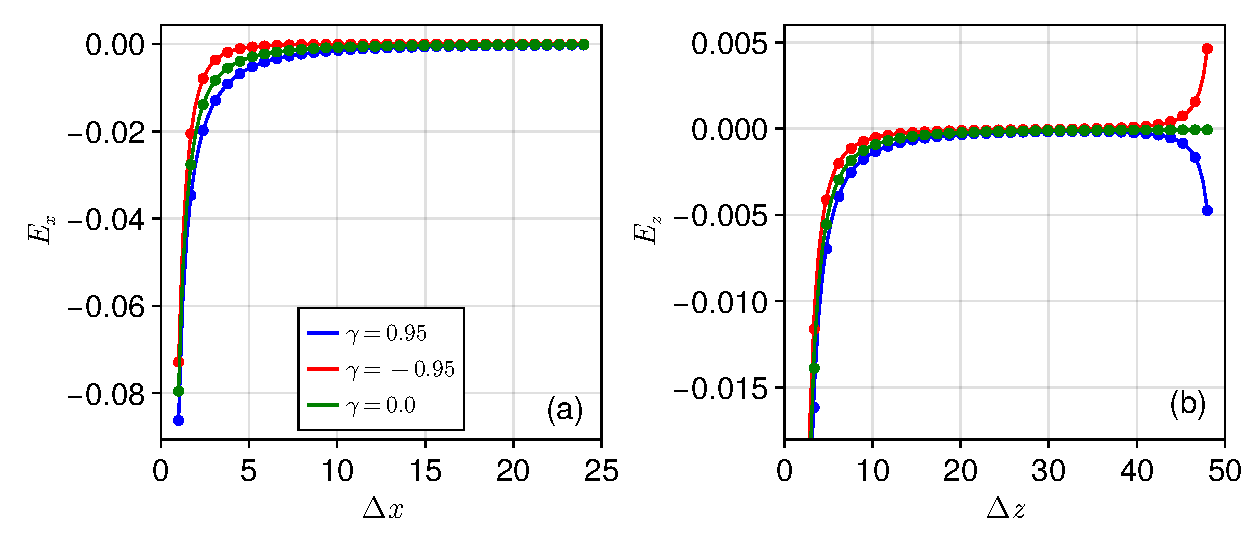
\includegraphics[width = \linewidth]{figs/E_xyz.pdf}
    \caption{
        Electric field in (a) $x$ and (b) $z$ between a pair of negatively charged particles, which are confined in a box with size of $(100, 100, 50)$.
        One of the particle is located at $(50, 50, 1)$, and the other one is located at (a) $(50 + \Delta x, 50, 1)$ and (b) $(50, 50, \Delta z)$.
        The lines are results by QEM and the dots are results by the ICM with direct lattice sum.
    }
    \label{fig:E_xyz}
\end{figure}

Then to validate the convergence of the QEM, we calculate the interaction energy of a system containing~$100$ randomly distributed particles using QEM, and the reference results are calculated by the ICM-Ewald2D method.
In Fig.~\ref{fig:Error_E}, the relative error of the interaction energy is plotted as function of the parameter~$E$ and the reflection rate~$\gamma$.
The results show that as $E$ increases, the relative error decreases rapidly, demonstrating the convergence of QEM.

\begin{figure}[htb]
    \centering
    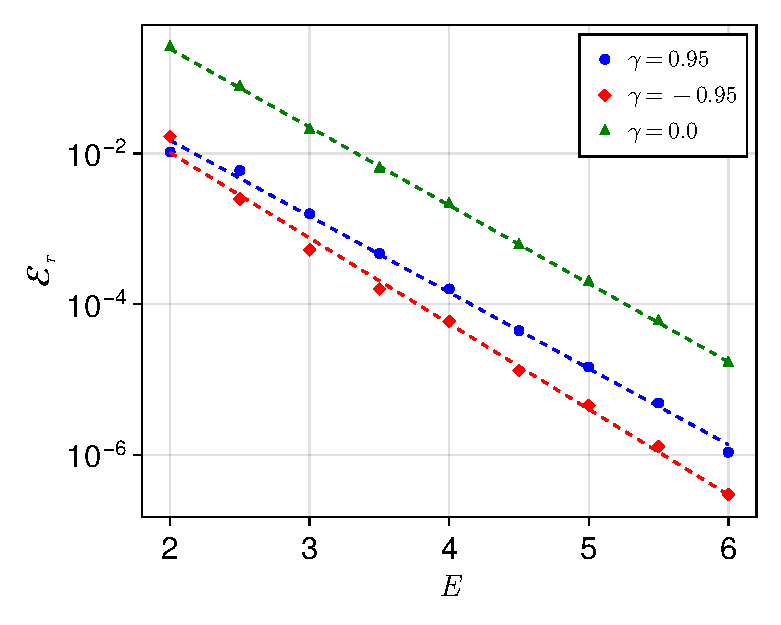
\includegraphics[width = 0.625\linewidth]{figs/e_total.pdf}
    \caption{
        Relative error of the energy of $100$ charged particles randomly distributed in a box with size of~$(100, 100, 50)$, as functions of the parameter~$E$ and reflection rates~$\gamma$.
    }
    \label{fig:Error_E}
\end{figure}


\subsection{Simulating electrolytes confined by dielectric interfaces}

To demonstrate the accuracy of the QEM for planar dielectric interfaces in a MD simulation, we study a few electrolytes modeled as the restricted primitive model, confined between two dielectric interfaces.
In all simulations, the box size is set as $(100 \tau_0, 100\tau_0, H)$, and consists of 436 particles immersed in continuum solvent characterized by a Bjerrum length $\ell_{\mathrm B} = e_0^2/(4 \pi \eps_c k_B T) = 3.5 \tau_0$, where~$e_0$ is the unit of smallest charge.
The ions are modeled as soft spheres of diameter~$\tau_0$ that have an excluded-volume interaction represented by a purely repulsive shifted-truncated Lennard-Jones (LJ) potential with energy scale~$\eps_{LJ} = k_B T$, where~$k_B$ is the Boltzmann constant and~$T$ is the absolute temperature.
The ions are confined by purely repulsive shifted-trunacted LJ walls ($\eps_\text{ion-wall} = k_B T$; $\tau_\text{ion-wall} = 0.5 \tau_0$) at $z = 0$ and $z = H$. 
The MD simulations is utilize a time step $0.001 t_0$, where $t_0 = \tau_0 m_0 / k_B T$ is the unit of time with $m_0 = 1$~(LJ unit), the ion mass, and temperature is controlled via Nosé–Hoover thermostat.
When evaluating the electrostatic interaction using the QEM, we set~$E = 4$,~$p = 30$ and~$n = 40$.
In all simulations, it takes~$2 \times 10^6$ time steps to reach equilibrium, after which we continue the simulation for $3 \times 10^6$ time steps for sampling.
We sample every 100 steps, which yields~$3 \times 10^{4}$ independent and equilibrated configurations.

\subsubsection{MD simulations of symmetric systems}

We first study symmetric systems where the top and bottom substrates have the same permittivity, i.e.,~$\gamma_u = \gamma_d = \gamma = \pm 0.95$, and we take~$H = 50 \tau_0$.
The system contains 218 cations and 218 anions carrying charge~$\pm e_0$, respectively.
To validate, we compared the charged distribution of QEM with result of the HSMA~\cite{liang2020harmonic}.
The ion density profiles by QEM and HSMA are shown in Fig.~\ref{fig:MD}, which shows that distributions obtained by QEM and HSMA overlap within statistical accuracy. 
The expected ion accumulation near high-permittivity surfaces and ion depletion near insulating interfaces are borne out by the simulations, which demonstrates that our method can accurately reproduce the characteristics of the system's equilibrium state.
The mean square displacements (MSD) in $xy$ and in $z$ of the simulation processes are shown in Fig.~\ref{fig:msd}.
The MSD in the periodic dimensions shown in Fig.~\ref{fig:msd}(a) is consistent with a normal diffusion process, where the~$O(t^2)$ and~$O(t)$ parts correspond to the short/long-time self diffusion, respectively.
Due to the confinements in~$z$, the MSD in the non-periodic dimension shown in Fig.~\ref{fig:msd}(b) behaves differently as a sub-diffusion process, where the MSD stop growing at long time, indicating the ions are confined by the dielectric interfaces.
The results here qualitatively agree well with that shown in previous experiments and simulations~\cite{das2010single, neusius2009subdiffusion}.

\begin{figure}[htbp]
    \centering
    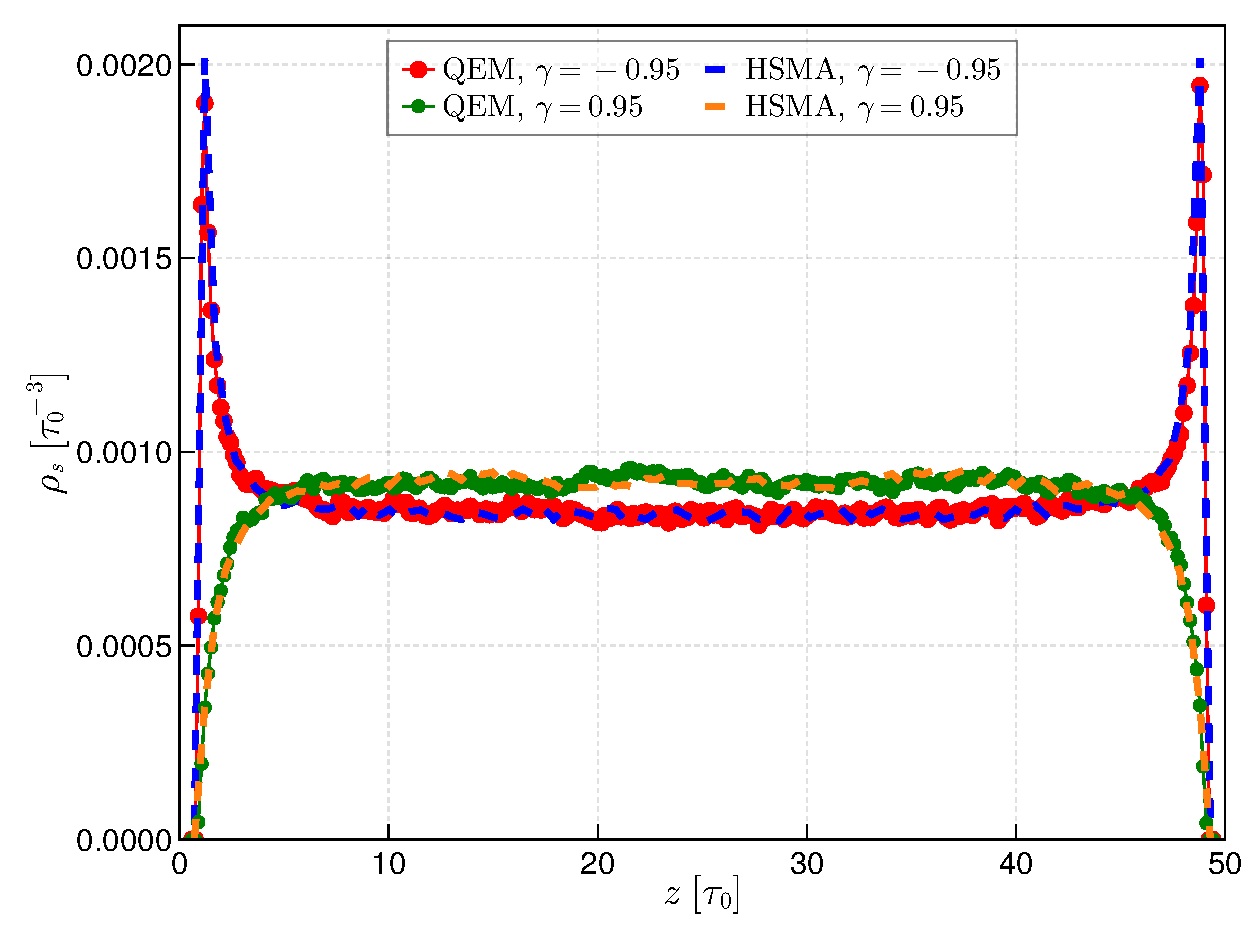
\includegraphics[width = 0.8 \linewidth]{figs/compare_HSMA.pdf}
    \caption{
        Distributions of ion density in~$z$ for symmetric electrolytes containing 218 cations and 218 anions and confined by neutral dielectric substrates with $\gamma_u = \gamma_d = \pm 0.95$ at~$z = 0$ and~$50\tau_0$, solid lines by QEM and dashed lines by HSMA.
    }
    \label{fig:MD}
\end{figure}

\begin{figure}[htbp]
    \centering
    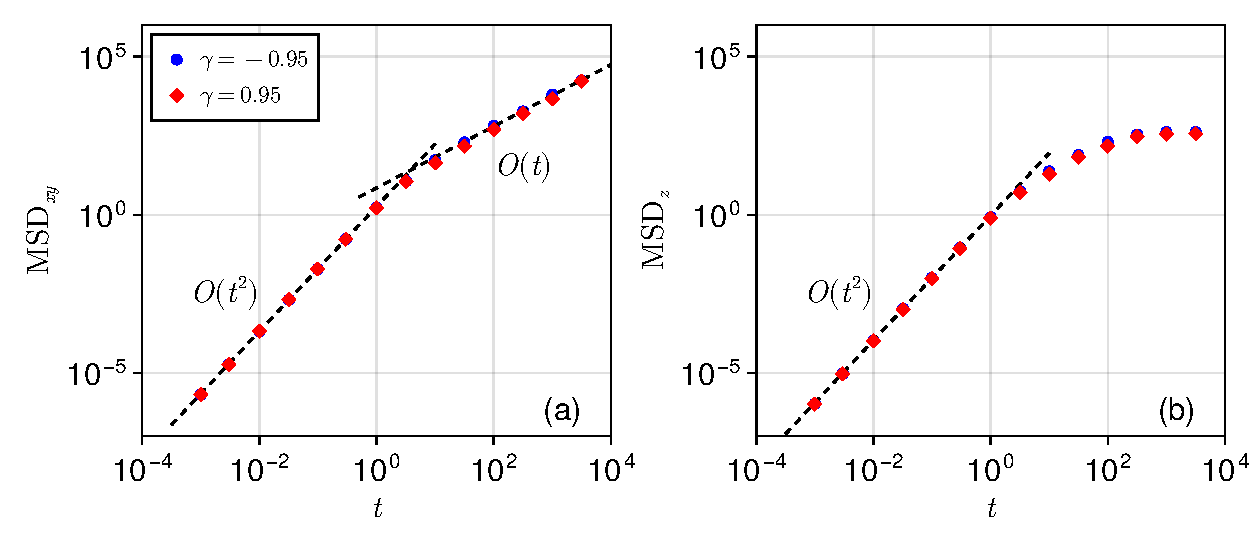
\includegraphics[width = 1.0 \linewidth]{figs/msd.pdf}
    \caption{
        The MSD of the ions in (a)~$xy$ and (b)~$z$, respectively, as functions of simulations time and reflection rates.
    }
    \label{fig:msd}
\end{figure}

Then CPU time for the QEM to compute the interactions between~$N$ particles is shown in Fig.~\ref{fig:timecost}, where cost of the Ewald2D method is also shown as reference.
The particle number surface density is fixed as~$4.36 \times 10^{-2} \tau_0^{-2}$ and thickness of the system is fixed to be~$50 \tau_0$, which are the same to the simulations above.
The number of charged particles is increased from~$10^2$ to~$10^5$.
For QEM, the same parameter as the previous simulations are applied; for Ewald2D method, parameter are selected so that the results are of 4-digit precision.
The results are shown in Fig.~\ref{fig:timecost}, which indicate that complexity of QEM is of~$O(N)$.

\begin{figure}[htb]
    \centering
    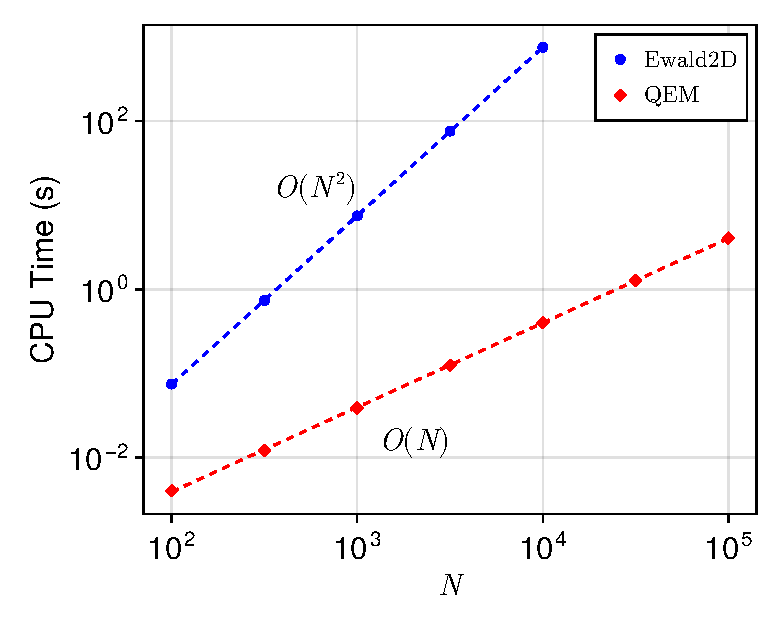
\includegraphics[width = 0.625\linewidth]{figs/runtime.pdf}
    \caption{
    CPU time of computing the interactions between all particles for different particle quantities under the condition of the same particle number surface density.
    The blue and red dots corresponding CPU time of Ewald2D method and QEM, and the dashed lines are fitted with slopes of~$2$ and~$1$, respectively.
    }
    \label{fig:timecost}
\end{figure}

\subsubsection{MD simulations of asymmetric systems}
As been mentioned above, QEM can be used to simulate asymmetric thin systems.
We consider two cases with asymmetry in dielectric mismatches and cation/anion valences.
In both cases, the thickness of the system is set as~$H = 10 \tau_0$, so that ~$L_{x/y} / H = 10$.

\textbf{Case I: Asymmetry in dielectric mismatches.}
In this case, we study the effect of the asymmetric dielectric mismatches.
The dielectric confinements are set as $\gamma_d = -0.95$ and~$\gamma_u = 0.95$, and the system contains 218 cations and 218 anions carrying charge~$\pm e_0$, respectively.
We keep other parameters the same as that of the previous example.

The spatial distribution of ions in~$z$ as shown in Fig.~\ref{fig:non_sym}.
Both cations and anions are attracted towards the lower dielectric plate with a negative reflection coefficient, while being repelled by the upper dielectric plate with a positive dielectric coefficient, thereby forming an strongly asymmetric spatial distribution as illustrated in Fig.~\ref{fig:non_sym}.

\begin{figure}[htbp]
    \centering
    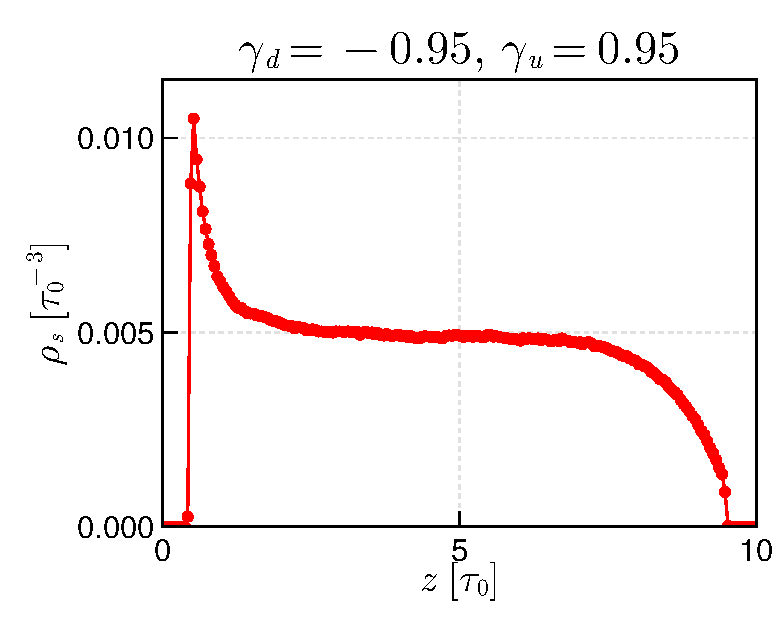
\includegraphics[width = 0.50\linewidth]{figs/non_symm.pdf}
    \caption{
        Ion density in~$z$ for symmetric electrolytes containing 218 cations and 218 anions and confined by neutral dielectric substrates with $\gamma_u = 0.95$,~$\gamma_d = -0.95$ at~$z = 0$ and~$10\tau_0$.
    }
    \label{fig:non_sym}
\end{figure}

\textbf{Case II: Asymmetry in cation/anion valences.}
Another application is the simulation of charge asymmetric systems.
In that simulation, we keep~$\gamma_u$ and $\gamma_d$ the same and equals to~$\gamma = \pm 0.95$, but simulate a $3:1$ salt with $109$ trivalent cations and $327$ monovalent anions. 
The other parameters are kept the same as above.

The results are shown in Fig.~\ref{fig:salt3-1}, which shows that the ion distributions are highly concentrated around the center or near the substrates.
For cations, due to the increase in the charge of the cations, the repulsive/attractive effects on both sides of the medium are significantly enhanced when~$\gamma$ greater or smaller than~$0$, respectively.
The anions are influenced by the distribution of cations, exhibiting characteristics of aggregation towards the center/sides, which are consistent with expectations.

\begin{figure}[htbp]
  \centering
  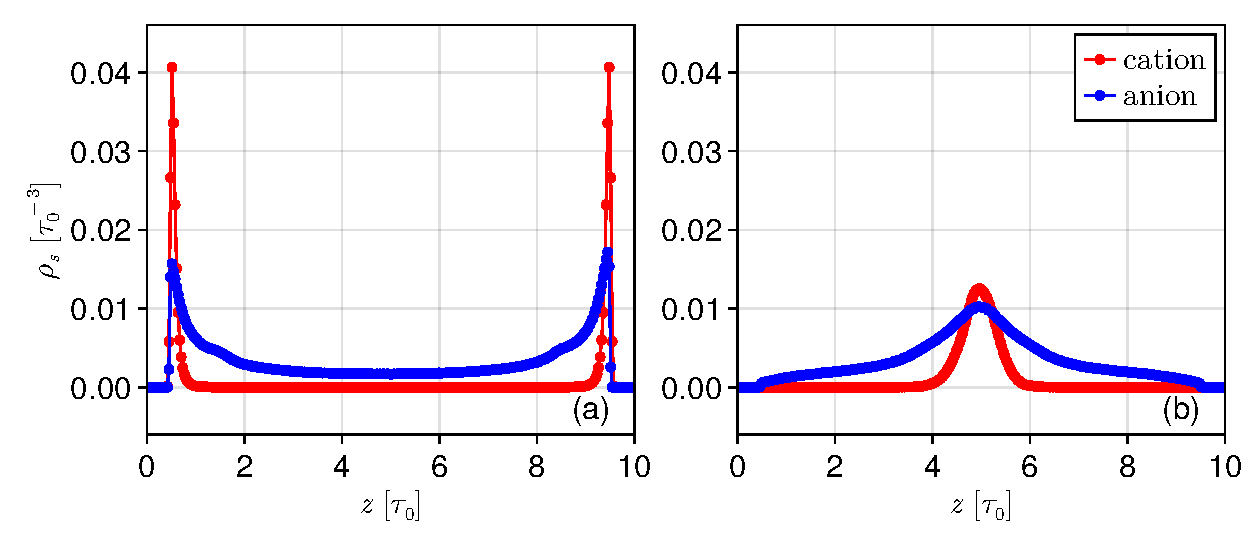
\includegraphics[width = \linewidth]{figs/density_3-1.pdf}

  \caption{
    Cation and anion density in~$z$ for a $3:1$ salt with $109$ trivalent cations and $327$ monovalent anions confined by neutral dielectric substrates with (a) $\gamma_u = \gamma_d = \gamma = - 0.95$ and (b) $\gamma_u = \gamma_d = \gamma = 0.95$.
    Red and blue lines are for cations and anions, respectively.
  }
    \label{fig:salt3-1}
\end{figure}

These cases indicates that QEM can also provide significant advantages in handling systems with particle asymmetry, thinness, and strong polarization effects.


\subsection{Oscillatory single particle field}

Applying the QEM to negatively confined systems, we find that the dielectric confinement effect turns out to be physically fascinating even in the presence of a single charged particle. 
In Fig.~\ref{fig:force_x} (a), we present the electric field in the $x$ direction generated by a cation with valence~$\nu=1$ located at~$(x_0, y_0, \tau_0)$ in a quasi-2D system with a thickness of~$10\tau_0$, as a function of the distance from the cation~$\Delta x=x-x_0$, for different reflection rates~$\gamma$ characterizing the confinement. 
The field is defined as~$-\nu\ell_B\partial_x G(\mathbf{r}, \mathbf{r_0})$, and~$\ell_B=e_0^2/(4\pi\epsilon_0\epsilon k_B T)$ is the Bjerrum length of the solvent, with~$e_0$ the elementary charge,~$\epsilon_0$ the vacuum permittivity,~$k_B$ the Boltzmann constant, and~$T$ the temperature. 
For~$\vert\gamma\vert<1$ cases, as illustrated by the blue ($\gamma=-0.95$) and orange ($\gamma=0.95$) lines in Fig.~\ref{fig:force_x} (a), the polarization weakens or enhances the bare Coulomb field ($\gamma=0$), but with no qualitative difference. 
The results obtained by our method are in good agreement with those obtained by ICM, shown in dots in Fig.~\ref{fig:force_x} (a). 
However, for~$\vert\gamma\vert>1$, the results become non-trivial and qualitatively different. 
At short distance ($\tau_0<\Delta x < 10\tau_0$), we observe from Fig.~\ref{fig:force_x}(a) a continuous transition in the the near field interaction from like-charge attraction (LCA) into repulsion as~$\gamma$ increases from $-10$ to $+10$,
which can be understood as a significant enhancement of the polarization effect for~$\abs{\gamma}<1$ cases.
Even more interesting is the far field, it no longer decays monotonically but exhibits oscillatory behavior, which is rarely reported in previous studies.

\begin{figure}[htbp]
	\centering
	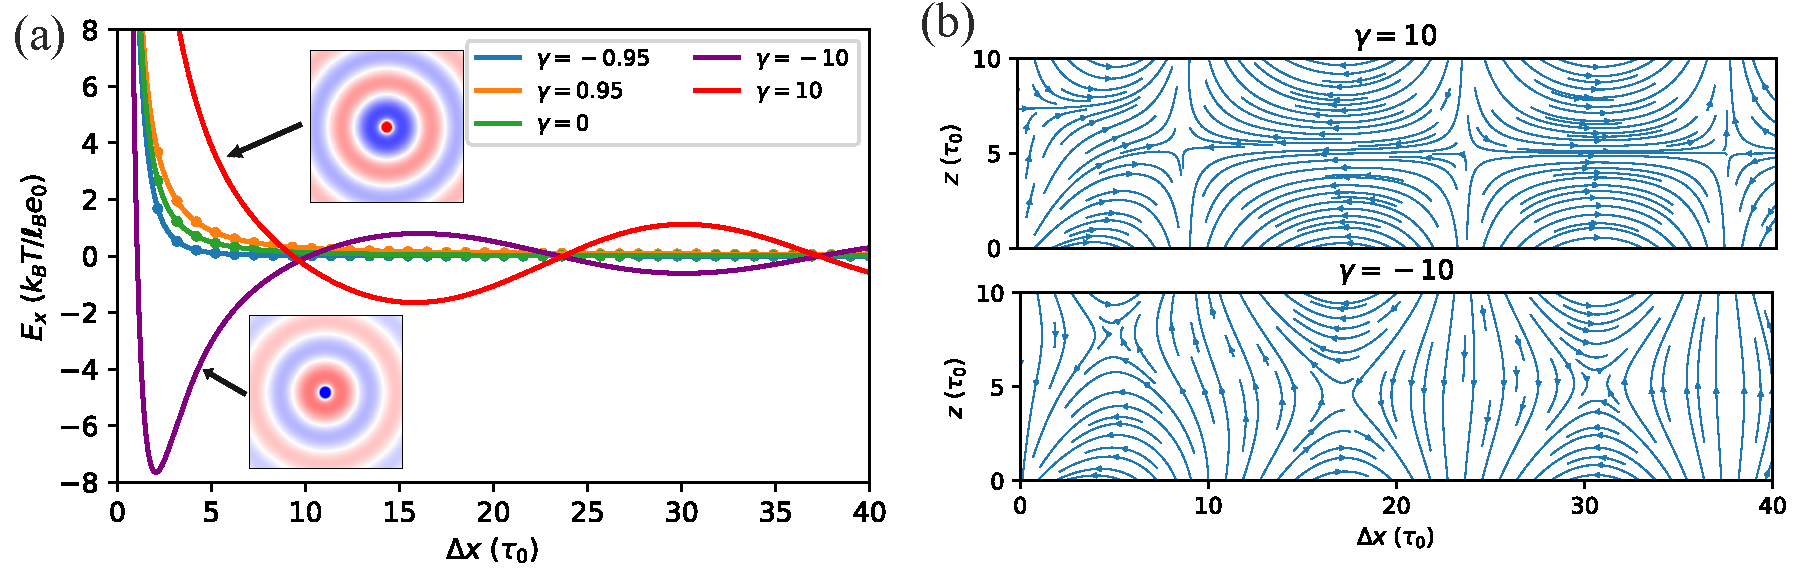
\includegraphics[width=1\textwidth]{figs/fig2.pdf}
	\caption{(a): the electric fields along~$x$ direction, generated by a cation with valence~$\nu=1$, fixed at~$z=\tau_0$, and confined by a pair of dielectric substrates located at~$z=0$ and~$10\tau_0$. Subplots depict the polarization charge density on the lower substrates. 
    (b): the corresponding field lines for the~$\gamma=\pm10$ scenarios.}
    \label{fig:force_x}
\end{figure}

To understand the origin of field oscillations, the polarization charge density profile on the substrate at~$z=0$ is shown in the subplots of Fig.~\ref{fig:force_x} (a).
The charge density is defined by 
\begin{equation}
    \sigma(\V{r}) = \lim_{z \to 0^+} \nu \ell_B \eps_0  \left( 1 - \frac{\eps}{\eps'} \right) \partial_z G(\V{r}, \V{r_0})\;,
\end{equation}
and the field lines generated by $\sigma(\V r)$ are sketched in Fig.~\ref{fig:force_x} (b). 
The field oscillation is found to be generated by the strong transverse polarization charge density waves, influencing both the near and far fields. 
The oscillatory field lines has a very similar structure to that of a surface plasmonic resonance wave~\cite{willets2007localized}, but the physical origin is different. 
The oscillation is due to the reflected polarization enhanced by the dielectric confinement, characterized by parameters~$\gamma_1$,~$\gamma_2$, and~$L_z$.
We observe that the wavelength of the oscillation, defined as two times the distance between nearby zeros, satisfies 
\begin{equation}\label{eq:wavelength}
    \lambda \cdot k_0 = 2 \pi \;,
\end{equation}
where~$k_0 = \frac{\ln{\gamma_1 \gamma_2}}{2 L_z}$ is the first-order pole in the Sommerfeld integral representation of the Green's function.
Numerical validation shows that Eq.~\eqref{eq:wavelength} is highly robust under different choices of~$\V{r}$,~$\V{r}_0$,~$\gamma$, or~$L_z$, as shown in Fig.~\ref{fig:k_wavelegth}.
Importantly, the oscillation fields can be accurately predicted and controlled by adjusting~$k_0$. 

\begin{figure}[htbp]
    \centering
    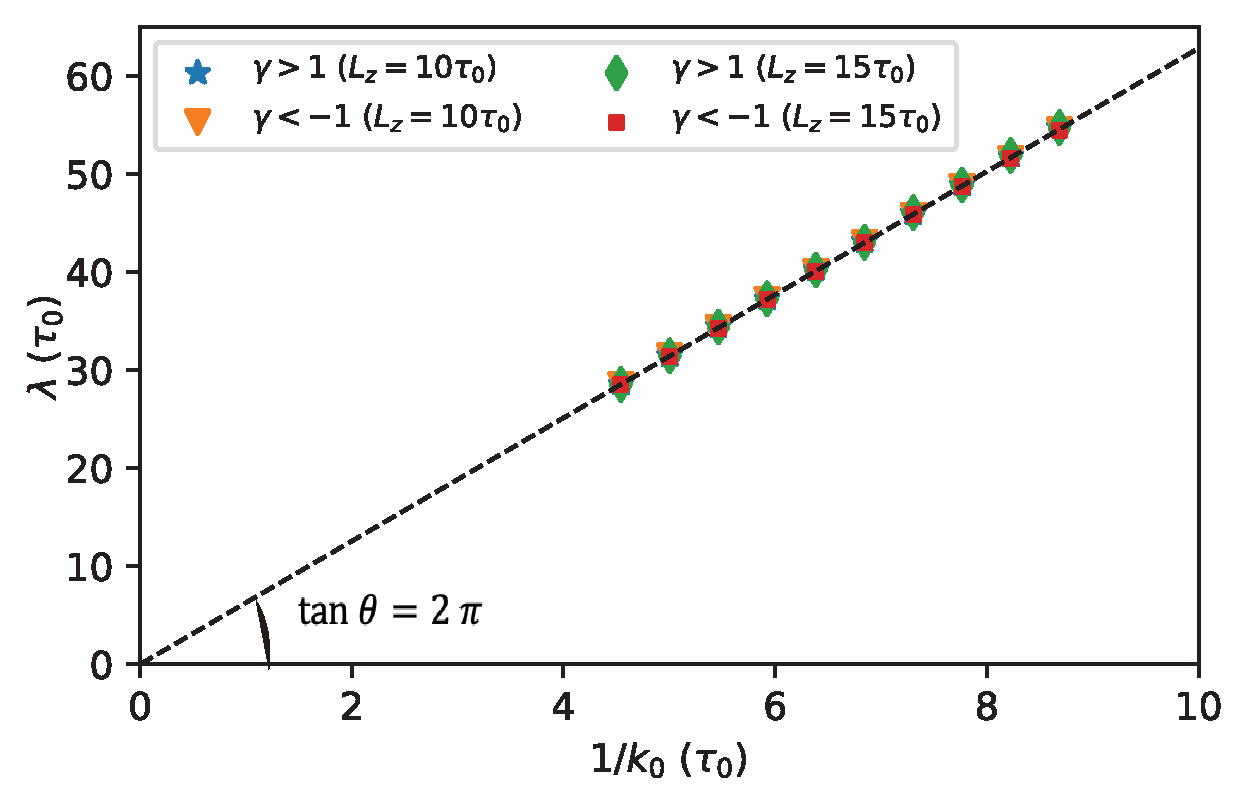
\includegraphics[width=0.6\textwidth]{figs/fig3.pdf}
    \caption{
        Numerical validations for the relationship between~$k_0$ and~$\lambda$ under various system parameter settings of~$\gamma$ and~$L_z$. For each case, $\lambda$ is approximated by averaging distances between nearby zeros of~$E_x$, and with different (randomly generated) locations in~$z$. 
    }
    \label{fig:k_wavelegth}
\end{figure}
